% siminos/blog/BuDiCv15blog.tex
% $Author: predrag $ $Date: 2017-03-17 00:22:06 -0400 (Fri, 17 Mar 2017) $
% Predrag moved reducesymm/blog/dailyBlogBB.tex to here     Nov 15 2013
% Predrag  switched to github.com                           Jul  8 2013
%           continues siminos/blog/dailyBlog.tex as of that date

% called in \chapter{Burak's notes} \label{c-dailyBlogBB}

\section{Burak's BuDiCv15 blog}
\label{sect-BuDiCv15blog}

% former siminos/ksRecycled/tex/blog.tex    master file: BuDiCv15.tex
\begin{description}
\item[2014-12-24 Burak] I just put together a rough outline for a paper on
\KSe\ and wrote little notes on how to fill it. \refFig{f-PCA} shows how
RPO and PPOs fill out the attractor in the PCA projection and on the
\PoincSec\ within this projection. \refTab{t-DynamicalAverages}
shows initial cycle averaging results obtained by ordering cycles with
respect to their topological lengths corresponding to the number of their
intersections with the Poinar\'e section in \reffig{f-PCA} (d). I added the
expansion up to order $N=8$, because at this order, it goes bad, flow
conservation and escape rate rule increases by one order, and observable
statistics stop converging. I'm planning to argue that at this level, we
are either missing some cycles, or we need a better topological ordering
method.

\item[2015-02-23 Burak] Making \reffig{f-PCA} (d) precise was a
little bit of an expensive calculation and it's cheaper if one
implements slicing in the post-processing. However, I found out that
when I count number of \PoincSec\ intersections from
post-processed trajectories, I found out that I get different
numerical results in the cycle expansions. I then checked carefully
and confirmed that if one does not sample \po s in slice time, then
one misses a few intersections with the Poincar\'e for multiple \po .
In other words, the border is a dynamically important region for
\KS\ dynamics and one really needs to use the slice time for
resolving it.

\item[2015-02-24 Burak] After discussion with Predrag I decided to
confirm that even though \fFslice\ does not reduce the continuous
symmetry of \eqva\ in second and third mode subspaces, the unstable
manifold of $EQ_2$ is unique since it is not on the \sliceBord ,
see \reffig{f-KSeq2manRefRed}. It does go in and outside the border
and that brings $\pi$-discontinuities, however, within the slice
the manifold is unique. I tried several different phase shifts and
plotted the one corresponds to shift by $pi/4$ in
\reffig{f-KSeq2manRefRed}.

\begin{figure}[ht]
\begin{center}
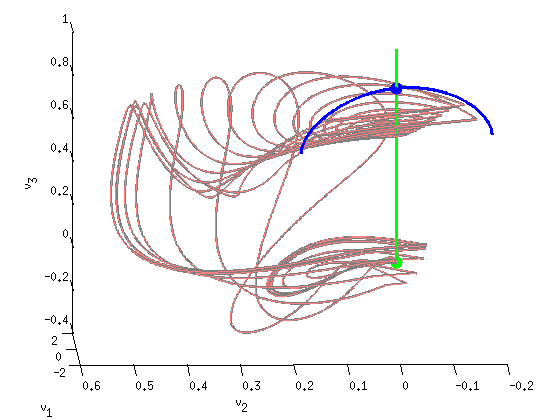
\includegraphics[width=0.60\textwidth]{KSeq2manRefRed}
\end{center}
\caption[]{
Unstable manifold of $EQ_2$ starting at two different (symmetry
equivalent) locations in the full \statesp (gray and red,
overlapping). Group orbits of $EQ_2$ and $EQ_3$ are green and blue
respectively.
}
\label{f-KSeq2manRefRed}
\end{figure}


\item[2015-02-26 Burak] After some thinking and experimenting, we
have arrived at the following conclusion regarding the unstable
manifold of $EQ_2$, and its homoclinic connection to its $L/4$
shifted location:

Even though the \fFslice\ does not reduce the symmetry of $EQ_2$,
its stable and unstable manifolds are unique in the \fFslice\
because those directions have non-zero first Fourier mode components.
\reffig{f-KSeq2manRefRed2} is same with \reffig{f-KSeq2manRefRed},
with addition three points within the slice:

\bea
    \mbox{black: } &&
    \OpSlice [ E_2 + \epsilon \, V_{1, E_2} ]
    \, , \continue
    \mbox{green: } &&
    \OpSlice [ E_2 + \epsilon \, V_{4, E_2} ]
    \, , \continue
    \mbox{blue: } &&
    \OpSlice [ E_3 + \epsilon \, V_{4, E_3} ] \, ,
\eea

where $\OpSlice$ is the ``slicing operator'' I defined in
\refeq{e-OpSlice},
$\epsilon = 10^{-6}$, and
$V_{1, E_2}$ is the unstable direction of
. So it basically means that the orbits which start
nearby the black dot (unstable direction of $E_2$) spiral out, some
of them gets close to the blue dot (stable direction of $E_3$) and
all of them ends up at the green dot (stable direction of $E_2$).

An important observation is that the difference between first Fourier
mode phases of $V_{2, \mbox{stable}}$ and $V_{2, \mbox{unstable}} $
is exactly $\pi/2$. This is consistent with the fact that in the full
\statesp\ this homoclinic connection is from $E_2$ to
$\tau_{1/4} E_2$ (see Fig 9 in \refref{SCD07}). So the distance
between green and black dots in \reffig{f-KSeq2manRefRed2} corresponds
to a quarter domain shift along the group orbit of $E_2$.

\begin{figure}[ht]
\begin{center}
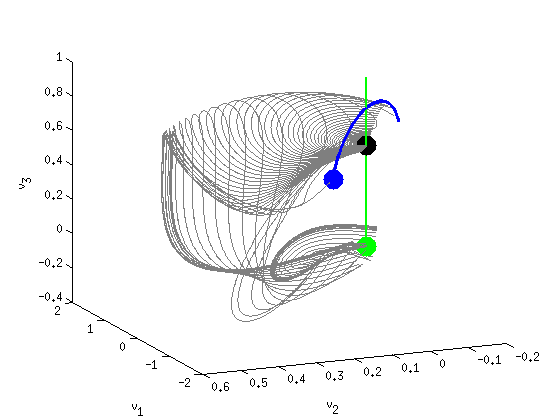
\includegraphics[width=0.60\textwidth]{KSeq2manRefRed2}
\end{center}
\caption[]{
Same with \reffig{f-KSeq2manRefRed}, but perturbations along the
stable (green) and unstable (black) directions of $E_2$ and stable
direction of $E_3$ (blue) are marked with dots. Discrete jumps due
to border visits are discarded for visibility.
}
\label{f-KSeq2manRefRed2}
\end{figure}

\item[2015-04-03 Burak] Another topic we discussed in the meeting
this week was the reflection-invariant dynamics of \KS\ system
at $L=22$. To start with this, I generated random
reflection-invariant initial conditions, and integrated them for
long times. \refFig{f-RefInv} shows outcome of such a simulation
in $PCA$ projection and in the configuration space. It seems like
orbits follow the intersection of $E_2$'s unstable manifold
which connects to $\LieEl (l = L/4) E_2$, with the reflection-invariant
subspace, and then bounce between $E_2$ and $\LieEl_{1/4} E_2$.
Time intervals of going back and fort changes in
\reffig{f-RefInv} but my guess is that it is due to build up of
numerical errors, but I'm not sure. This is a speculation, but
I think that there can be infinitely many periodic orbits in this
subspace, which would connect the stable and unstable manifolds of
$E_2$ and $\LieEl (l = L/4) E_2$ respectively and vice versa. I think
we should somehow use this information in cycle expansions because
the reflection invariant dynamics sits right in the middle of the
attractor.

\begin{figure}[ht]
\begin{center}
    (a) 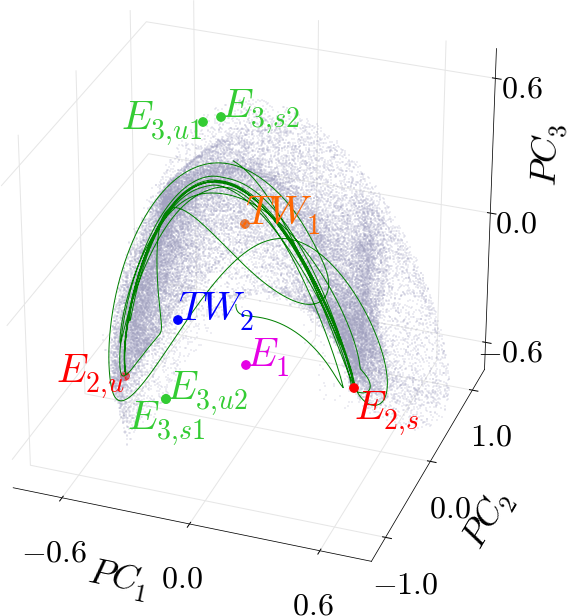
\includegraphics[width=0.45\textwidth]{ksRefInvPCA}
    (b) 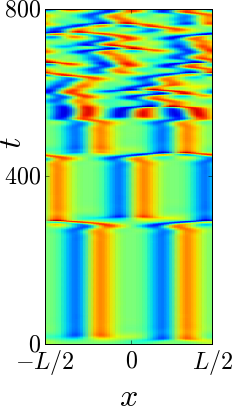
\includegraphics[width=0.25\textwidth]{ksRefInvConf}
\end{center}
    \caption[]{
        \KS\ dynamics in the reflection-invariant subspace,
        starting from a random initial condition, until falls
        onto the strange attractor due to build up of
        numerical errors.
        (a) PCA projection (green trajectory).
        (b) Configuration space.
    }
    \label{f-RefInv}
\end{figure}

\item[2015-04-06 Burak] Interesting looking dynamics in
\reffig{f-RefInv} turned out to be numerical error. Once I restricted
the integrator to stay in the reflection invariant subspace, $E_2$
became stable and attracted all trajectories. \refFig{f-RefInvConf}
shows two trajectories starting from unstable manifolds of $E_2$ and
$E_3$ and they both converge to $E_2$ and stay there.

\begin{figure}[ht]
\begin{center}
    (a) 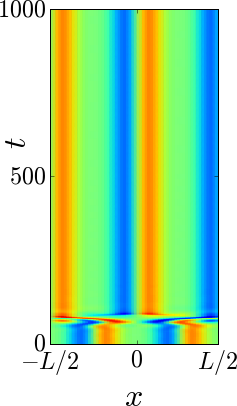
\includegraphics[width=0.25\textwidth]{ksRefInvConfeq2}
    (b) 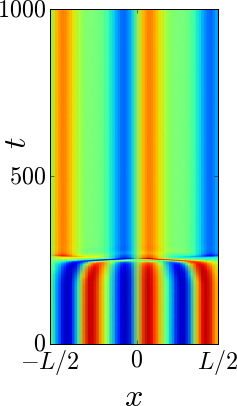
\includegraphics[width=0.25\textwidth]{ksRefInvConfeq3}
\end{center}
    \caption[]{
        \KS\ dynamics in the reflection-invariant subspace,
        starting from a random the unstable manifolds. of $E_2$ (a)
        and $E_3$ (b).
    }
    \label{f-RefInvConf}
\end{figure}

\item[2015-4-6 Xiong] I run a rather long simulation of total 1000
different orbits with random initial condition to obtain
average dissipation and its variance. The result is shown
in \reffig{fig:averD} and \reffig{fig:averD2}. The former
converges very well, but the latter has relatively large
variation.

\begin{figure}[ht]
\begin{center}
  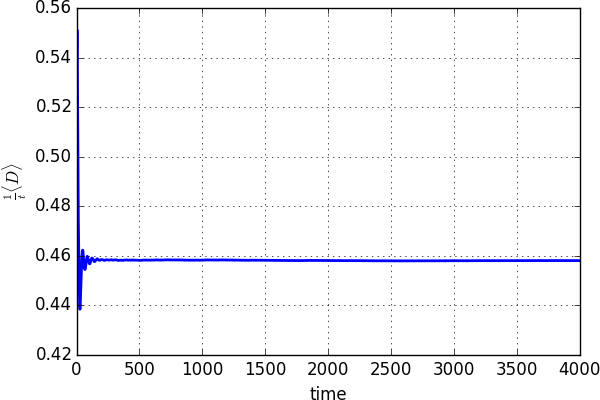
\includegraphics[width=0.5\textwidth]{ksD}
\end{center}
  \caption{average dissipation, $0.4583\pm 0.0005$.}
  \label{fig:averD}
\end{figure}
\begin{figure}[ht]
\begin{center}
  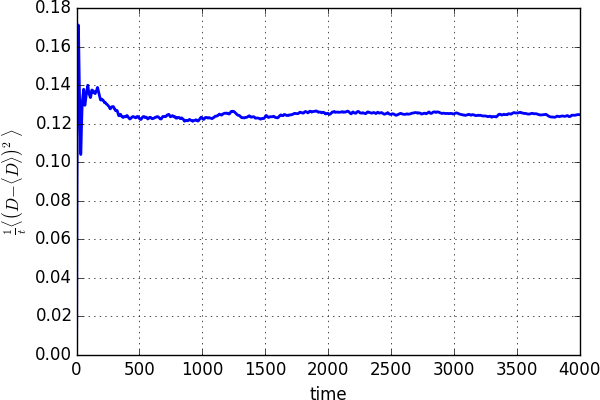
\includegraphics[width=0.5\textwidth]{ksD2}
\end{center}
  \caption{variance of dissipation, $0.124\pm 0.003$.}
  \label{fig:averD2}
\end{figure}
\begin{figure}[ht]
\begin{center}
  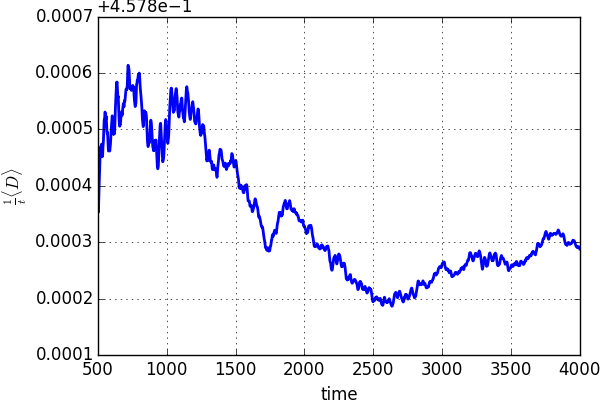
\includegraphics[width=0.4\textwidth]{ksD3}
  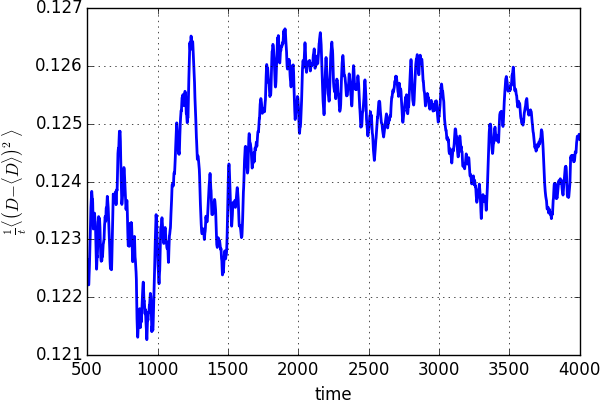
\includegraphics[width=0.4\textwidth]{ksD4}
\end{center}
  \caption{average dissipation and variance of dissipation. Data for $T < 500$
  is not shown.}
  \label{fig:averD3}
\end{figure}

\item[2015-04-06 Burak] Since we have a poor convergence of the cycle
expansions, I decided to plot distribution of leading Floquet exponents
with respect to the topological lengths determined from
\reffig{f-Poincare}. These plots are in \reffig{f-FloquetExps}. My
current conclusion is my heuristic cycle ordering was just a bad idea.
I'll try stability ordering and other things starting from tomorrow.

\begin{figure}[ht]
\begin{center}
    (a) 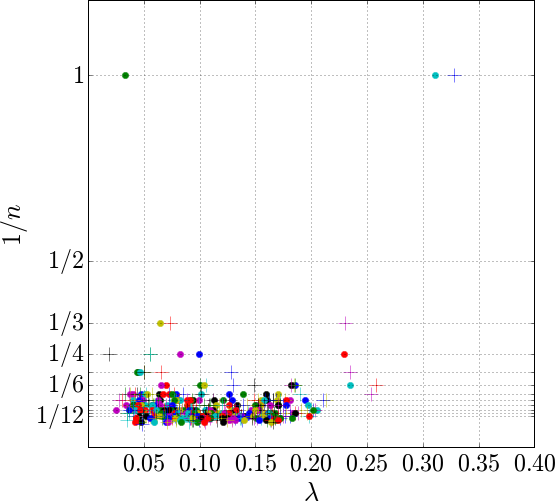
\includegraphics[width=0.40\textwidth]{ksFloquetExpsTopLength}
    (b) 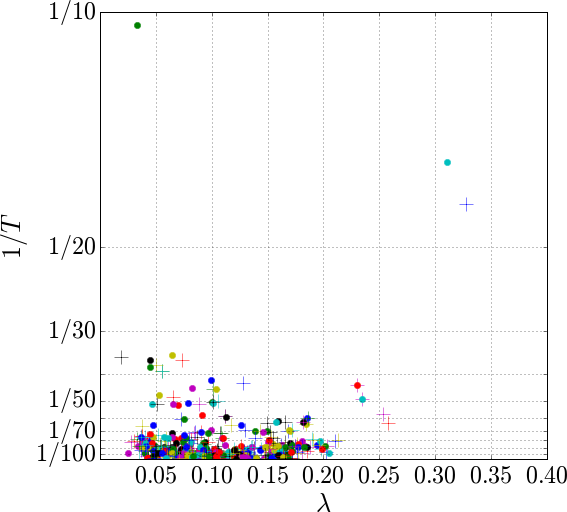
\includegraphics[width=0.40\textwidth]{ksFloquetExpsPeriod}
\end{center}
    \caption[]{
        Distribution of leading Floquet exponents with respect to
        topological lengths determined from \PoincSec\ of
        \reffig{f-Poincare} (a) and cycle periods (b). In both figures,
        RPOs marked with `+'s and PPOs marked with `.'s.
    }
    \label{f-FloquetExps}
\end{figure}

\item[2015-04-06 Burak] I started looking at PCA projections other than
the first three and found out that projections on $(PC_4, PC_5, PC_6)$
reveals shadowing of the periodic orbits.
Green orbit in \reffig{f-ppo10p3rpo32p8PCA} is the shortest PPO with
period $T=10.3$ and the red one is the second shortest \RPO{2} with period
$T=32.8$. What's interesting is while the two orbits seems far from
each other in \reffig{f-ppo10p3rpo32p8PCA} (a), they seem to overlap
for a long period in \reffig{f-ppo10p3rpo32p8PCA} (b). To get a better
intuition, look at the configuration space plots of these orbits in
\reffig{f-ppo10p3rpo32p8conf}. $PPO_{10.3}$ (a) can be described as two
wiggly peaks and two less wiggly peaks, where more wiggly peaks
shift a quarter domain at each period. Now if you look at
\reffig{f-ppo10p3rpo32p8conf} (b), at time $t = 20$, $\RPO{2}=RPO_{32.8}$ does
a very similar thing where peaks on the left doesn't move much, peaks
on the right shift a quarter domain. This behavior is different then
what happens in the unstable manifold of $E_2$ where all peaks shift a
quarter domain.

There are many other orbits, which appear to be shadowed by
$PPO_{10.3}$, thus, it is a primary task to understand the unstable
manifold of this orbit.
Unfortunately, leading Floquet multiplier of $PPO_{10.3}$ is a complex
pair, so it is going to be challenging to visualize it, but I'll try.

\begin{figure}[ht]
\begin{center}
    (a) 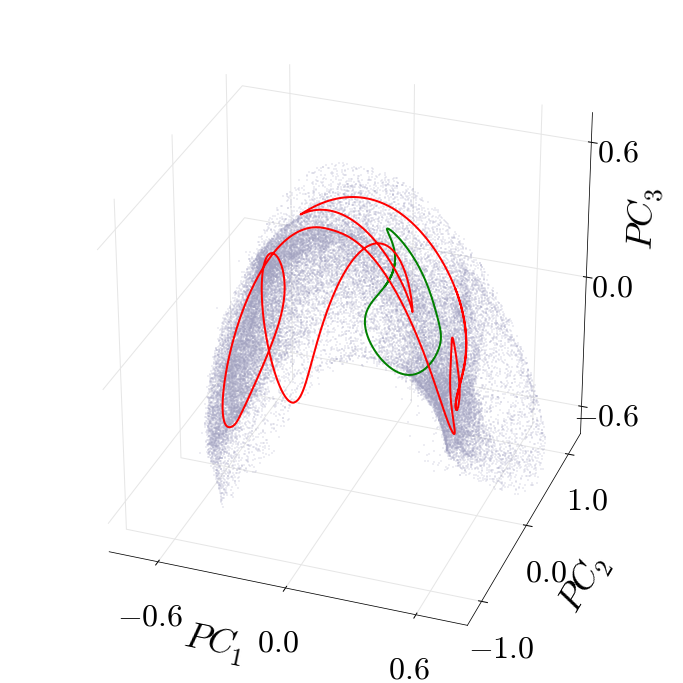
\includegraphics[width=0.40\textwidth]{ksPCA13ppo1rpo2}
    (b) 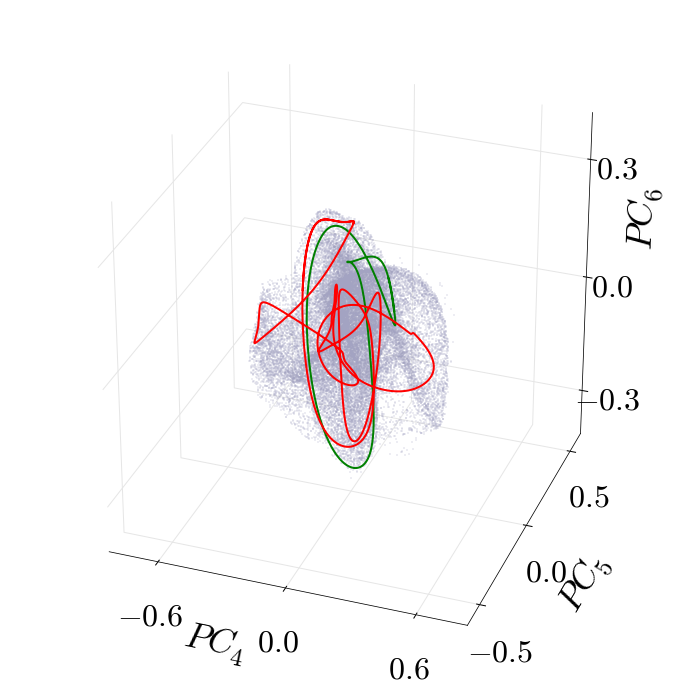
\includegraphics[width=0.40\textwidth]{ksPCA46ppo1rpo2}
\end{center}
    \caption[]{
        \RPO{2} (T = 32.8) (red) and PPO (T = 10.3) along with the ergodic
        cloud projected onto (a) $(PC_1, PC_2, PC_3)$,
        (b) $(PC_4, PC_5, PC_6)$
    }
    \label{f-ppo10p3rpo32p8conf}
\end{figure}

\begin{figure}[ht]
\begin{center}
    (a) 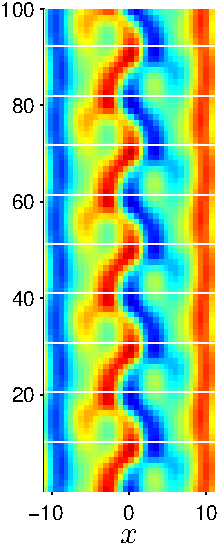
\includegraphics[width=0.20\textwidth]{ks22ppo10p3}
    (b) 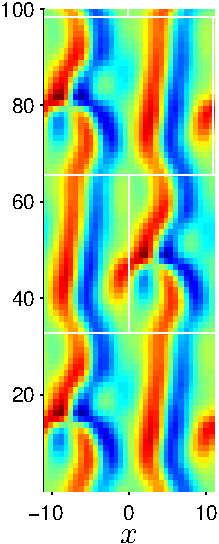
\includegraphics[width=0.20\textwidth]{ks22rpo032p8}
\end{center}
    \caption[]{
        \RPO{2} (T = 32.8) (a) and PPO (T = 10.3) (b) in configuration
        space.
    }
    \label{f-ppo10p3rpo32p8PCA}
\end{figure}

\item[2015-04-18 Burak] As I was failing at constructing the unstable
manifold of $PPO_{10.3}$, I realized that if I change the initial
condition $\ssp_{0}$ of the $PPO$ by a continuous shift
$\LieEl (\theta)$, the $PPO$ no longer arrived at a
reflection transformed location after one period, but closed onto
itself after two. I showed it to Xiong Ding, and he immediately
solved the mystery. A $PPO$ satisfies:
\beq
    \flow{\period{p}}{\sspPPO (0)} = \matrixRep (R) \sspPPO (0)   \, ,
    \label{e-PPOevolve}
\eeq
Now if we shift this state by $\theta$, its evolution becomes
\bea
    \flow{\period{p}}{\matrixRep (\LieEl (\theta ) ) \sspPPO(0)} &=&
        \matrixRep(\LieEl(\theta)) \flow{\period{p}}{\sspPPO(0)} \, ,
            \label{e-shiftPPOeqv} \\ &=&
        \matrixRep(\LieEl(\theta)) \matrixRep (R) \sspPPO (0) \, ,
            \label{e-shiftPPOevolve} \\ &=&
        \matrixRep (R) \matrixRep(\LieEl(- \theta)) \sspPPO (0) \, ,
            \label{e-shiftPPOnoncommute}
\eea
where \refeq{e-shiftPPOeqv} followed from the equivariance,
\refeq{e-shiftPPOevolve} followed from \refeq{e-PPOevolve}, and
sign change in \refeq{e-shiftPPOnoncommute} is a consequence of
non-commutativity of reflection and $\SOn{2}$ rotations. Thus if we
$\SOn{2}$ rotate a $PPO$ by $\theta$, after one period, it picks up
a $-2$ times the phase shift along with the reflection after one
period, i.e. define
$\sspPPO' = \matrixRep (\LieEl (\theta ) ) \sspPPO(0)$,
\beq
    \flow{\period{p}}{ \sspPPO' } =
        \matrixRep (R) \matrixRep(\LieEl(- 2 \theta)) \sspPPO' \, ,
       \label{e-rotateppo}
\eeq
hence the Floquet matrix for this orbit is
\beq
    \jMps_p (\sspPPO') = \matrixRep (R) \matrixRep(\LieEl(- 2 \theta))
                         \left.
                         \frac{d \flow{\period{p}}{ \ssp }}{d \ssp}
                         \right|_{\ssp = \sspPPO'} \, .
   \label{e-JPPOshift}
\eeq

\item[2015-04-20 -- 22 Burak] \refFig{f-ppo10p3UnstMan} is the first visualization of
the unstable manifold of $PPO_{10.3}$. I'll first explain how I produce this
figure:

First of all, we have to work in the fully reduced \statesp\ \refeq{e-sspRefRed},
for which we first need to transform to the \fFslice . However, as I explained
in my previous post ([2015-05-18]), when subjected to a continuous shift,
pre-periodic orbits pick up an $\SOn{2}$ phase after one period, hence I had
to recompute their Floquet spectrum by computing eigenvalues of
\refeq{e-JPPOshift}. Leading Floquet multiplier for $PPO_{10.3}$ is

\beq
   \Lambda = -0.594985402952045 \pm 1.273494012917033i
\eeq

So its unstable manifold has two transverse directions. In order to visualize
this manifold, we need to transform corresponding eigenvector $V_1$ first
to the slice, and then to the reflection-reduced coordinates. Transformation
to the slice is done by Xiong's projection operator (see Lyapunov blog)
\bea
   \hat{V}_1 &=& h(\sspRed) V_1 \, , \\
   &&\mbox{where } h(\sspRed)=
       \matId-\frac{\ket{\groupTan(\sspRed)}\bra{\sliceTan{}}}
       {\braket{\groupTan(\sspRed)}{\sliceTan{}}}
\eea
and then transformation to the reflection reduced coordinates is done by
multiplying by the Jacobian of the transformation to \refeq{e-sspRefRed}
from the \fFslice
\beq
   \tilde{V}_1 = \Gamma_{\sspRed} V_1 \, .
\eeq
We transform the velocity vector to the reflection-reduced coordinates similarly
\beq
   \velRefRed(\sspRefRed) = \Gamma_{\sspRed} h(\sspRed) \vel(\sspRed) \, .
\eeq
I use the velocity vector $\velRefRed(\sspRefRed)$ as the \PoincSec\ normal.
The Floquet vector is projected to this \PoincSec\ as
\beq
   \tilde{V}_{1, PS} = \left(
                   \matId
                  -\frac{\ket{\velRefRed(\sspRefRed)}\bra{\velRefRed(\sspRefRed)}}
                       {\braket{\velRefRed(\sspRefRed)}{\velRefRed(\sspRefRed)}}
                  \right)
                  \tilde{V}_1 \, .
\eeq
$\tilde{V}_{1, PS}$ is orthogonal to $\velRefRed(\sspRefRed)$ by construction.
I construct the basis $e_{1, 2}$ for the \PoincSec\ by
Gram-Schmidting real and imaginary parts of the $\tilde{V}_{1, PS}$.
I then start $N_{\mu} \times N_{\phi}$ orbits according to the following rule
\bea
   \sspRefRed_{l, m} &=& \sspRefRed_{PPO, 0} + \epsilon \, e^{l  \frac{T \mu}{N_{\mu}}}
                     \, \left\{
                     \cos(m 2 \pi / N_{\phi}) \, Re[\tilde{V}_{1, PS}]
                  +  \sin(m 2 \pi / N_{\phi}) \, Im[\tilde{V}_{1, PS}] \
                         \right\} \, , \continue
                    && \mbox{where }
                       l = 1, \ldots \, , N_{\mu} \, , \,
                      m = 1, \ldots \, , N_{\phi} \, \, ,
   \label{e-ComplexUnstMan}
\eea
integrate for a time $t_f$, and mark the intersections. It is
essential that the vectors appearing in \refeq{e-ComplexUnstMan} are
real and imaginary parts of the Floquet vector in the \PoincSec,
not the orthonormalized basis vectors constructed from them.
The linearized manifold is organized as an expanding ellipse, not a
circle.

\refFig{f-ppo10p3UnstMan} is generated using
$\epsilon = 10^{-6}, N_\mu = 40, N_\phi = 36, t_f = 395$.


\begin{figure}[ht]
\begin{center}
    (a) 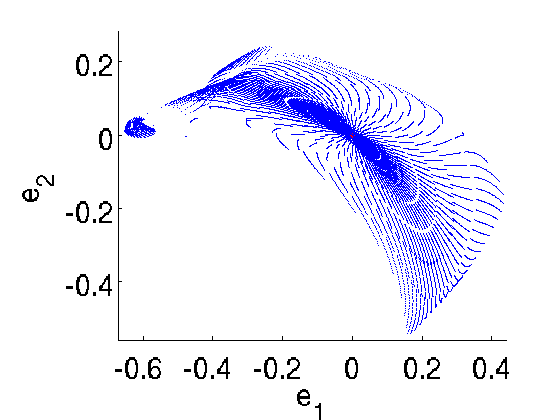
\includegraphics[width=0.40\textwidth]{ksPPO10p3Poincare}
    (b) 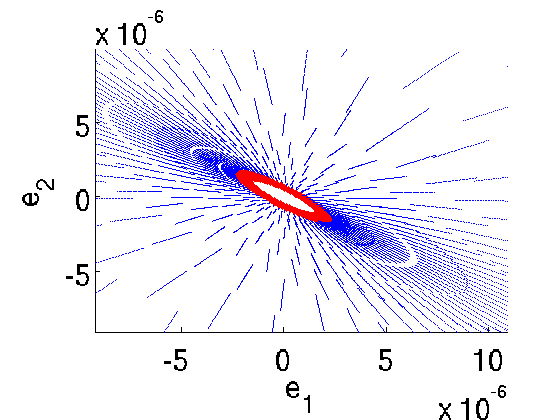
\includegraphics[width=0.40\textwidth]{ksPPO10p3PoincareZoom}
\end{center}
    \caption[]{
        (a) Unstable manifold of PPO (T = 10.3) on the \PoincSec\
        perpendicular to the velocity field, projected onto the plane
        spanned by the real and imaginary components of the leading Floquet
        vector. (b) Same as (a), zoomed in to the neighborhood of the origin.
    }
    \label{f-ppo10p3UnstMan}
\end{figure}

\item[2015-04-29 Burak] I computed the stability ordered zeta function
and cycle averages using it and results look like garbage, so I don't
see a reason for blogging them for now. However, as I was looking at
the periodic orbit data, suspiciously close number caught my eye for
RPOs with $T=36.2$, which stand at the 5th and 6th place in the RPO
database. They have same period and Floquet exponents with 6 significant
digit agreement and their trajectories in PCA projection looks like
\reffig{f-ksRPO5n6}. Their features are entirely same, and their slight
difference is I believe due to different starting points and different
build up of the integration errors. So I'm pretty sure that these two
are the same orbit. The reason both of them sneaked into the database
is probably the inaccuracies of the previous eigenvalue calculation.
Xiong is going to check his database for possible duplicates similar to
this, and then I'll get back to cycle expansion calculations as soon as
I make sure that we don't have duplicates. These by the way are pretty
short orbits, and had probably been messing up all cycle expansion
calculations.

\begin{figure}[ht]
\begin{center}
    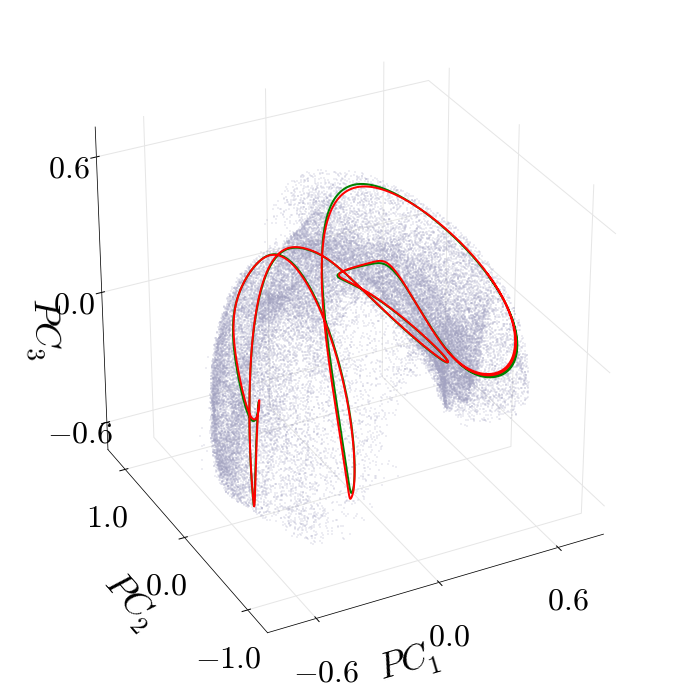
\includegraphics[width=0.40\textwidth]{ksRPO5n6}
\end{center}
    \caption[]{
      5th and 6th RPO from the database with same (6 agreeing digits)
      period and Floquet multipliers.
    }
    \label{f-ksRPO5n6}
\end{figure}

\item[2015-04-30 Ruslan] You need to double check this.  The 5th and
6th orbits were similar, but not the same in the earlier versions of
the database, but they are now the same and equal to the 6th in the
earlier database.  Maybe the 5th one was somehow overwritten by the
6th in the updated database?

\item[2015-04-30 Xiong to Ruslan] You are right. The new database is
obtained by my refinement of your original data for shorter time step.
I only have the initial
conditions of 5th and 6th rpo, not a set of shooting points along these
two orbits, so my Levenberg - Marquardt shooting method fails to distinguish
them. Do you have the original data of their shooting points ?
Also for
pairs (ppo108, ppo120) and (ppo146, ppo147), they are different
pre-periodic orbits. That is true,  but they are
related by rotation by $\pi$
as shown in \refeq{e-rotateppo}, should we include
them in the database?

\item[2015-04-30 Xiong] The correct rpo5 and rpo17 are refined from
Ruslan's data. These two orbits are sensitive to the Newton iteration
number. Previous calculation used too many steps.

\item[2015-05-08 Ruslan to Xiong] You can generate the shooting
points using ksfmstp2.m in matlab/ruslan.  Whether or not you'll get
convergence with the smaller step I don't know.  Most of the orbits
I found with $h=0.25$, I also checked with $h=0.1$ and they were
distinct. But obviously this is not a guarantee that it will remain
so in the limit $h \to 0$.  To be more sure, you might have to
generate a sequence of converged rpos/ppos with decreasing $h$.
Reviewing my data, I'm quite confident that rpo5 and rpo6 are
approximations of distinct rpos.  Same for ppo108 and ppo120.  For
ppo146/ppo147 you might be right that this is the same ppo shifted
by $\pi$.  Overall, even if there are some duplicates, I don't
believe they will have a significant effect on your cycle
expansions.  I believe that much more significant will be the
absence of rpos/ppos which we did not manage to detect.

\item[2015-05-08 Xiong to Ruslan] Yes, you are right. Predrag told me
before that some PO pairs come from bifurcation, so they have different
stability, but I forgot.

\item[2015-05-08 Xiong to Burak] I doubled the time step and divided
time step by 5, the long time simulation of dissipation and its variance
still look like \reffig{fig:averD3}, almost in the same range, so I do
not upload the new figures.

\item[2015-05-14 Burak] \emph{A question to Predrag and Xiong:}

I have so far been not very lucky in computing cycle expansions for
\KS\ system, and I ended up being convinced that without really
understanding the structure of the flow, and being sure that we
really know all the periodic orbits up to some period, it's unlikely
to make good cycle expansion calculations. However, there is still
material here, namely the complete \On{2} reduction, which I believe
is worthy to publish. So I thought we can illustrate the utility of
a fully reduced representation by showing the shadowing between a
pre-periodic and a relative periodic orbit. My intuition from \reffig
{f-ppo10p3rpo32p8conf} is that $\RPO{2}=\RPO{32.8}$ and $PPO_{10.3}$ are
good candidates for this purpose and we could probably show that
their unstable manifolds align for a certain period. We can probably
show this by plotting their Floquet vectors along the orbits and
illustrate that they do align during the shadowing episodes.

What are your opinions about this? If you agree, Xiong can teach me how
to compute Floquet vectors at different places, and I'll figure out
their transformation to the fully reduced space and do some
experiments hopefully will not take too long to produce something
meaningful.

\begin{figure}[ht]
\begin{center}
    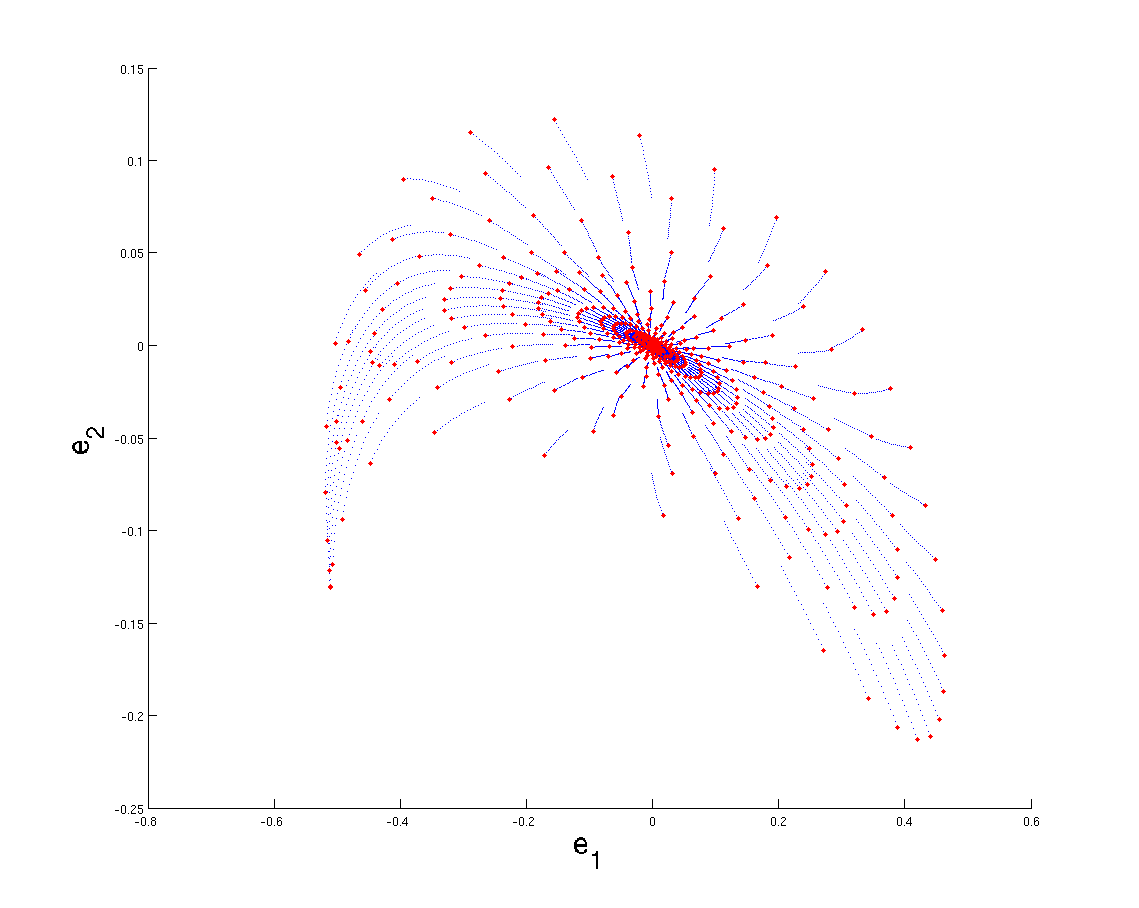
\includegraphics[width=0.60\textwidth]{ksPPO10p3Poincare2}
\end{center}
    \caption[]{
      Same as \reffig{f-ppo10p3UnstMan} (a), on a different location on
      the PPO, $\epsilon = 10^{-6}$, 36 returns.
    }
    \label{f-ppo10p3UnstMan2}
\end{figure}

\item[2015-05-26 Burak] I am going to try computing and visualizing
three dimensional unstable manifold of $PPO_{10.3}$ by computing it at
different locations on the orbit and then connecting end points until
the manifold folds. In \reffig{f-ppo10p3UnstMan2}, I plotted this
manifold on the \PoincSec\ after 36 returns and I marked red
each intersection corresponding to $l = N_\mu$ in
\refeq{e-ComplexUnstMan}. This could be something we can present as an
application of the symmetry reduction.

\item[2015-05-28 Burak] I decided to look at the unstable manifold
\reffig{f-ppo10p3UnstMan2} of $PPO_{10.3}$ in three dimensions, and
found out that it traverses a huge volume in the \statesp . In
\reffig{f-ksPPO1man3D}, the gray volume corresponds to the 384 orbits
which are organized as in the \PoincSec\ of
\reffig{f-ppo10p3UnstMan2}. I was expecting to see a tube of orbits
rotating around the $PPO_{10.3}$ (red in \reffig{f-ksPPO1man3D}), but I
found that they go all over the place, yet come back to the \PoincSec\
in a regular fashion. Furthermore, $\RPO{2}=\RPO{32.8}$ (green in
\reffig{f-ksPPO1man3D}) seems to follow this manifold at several places.

\begin{figure}[ht]
\begin{center}
    (a) 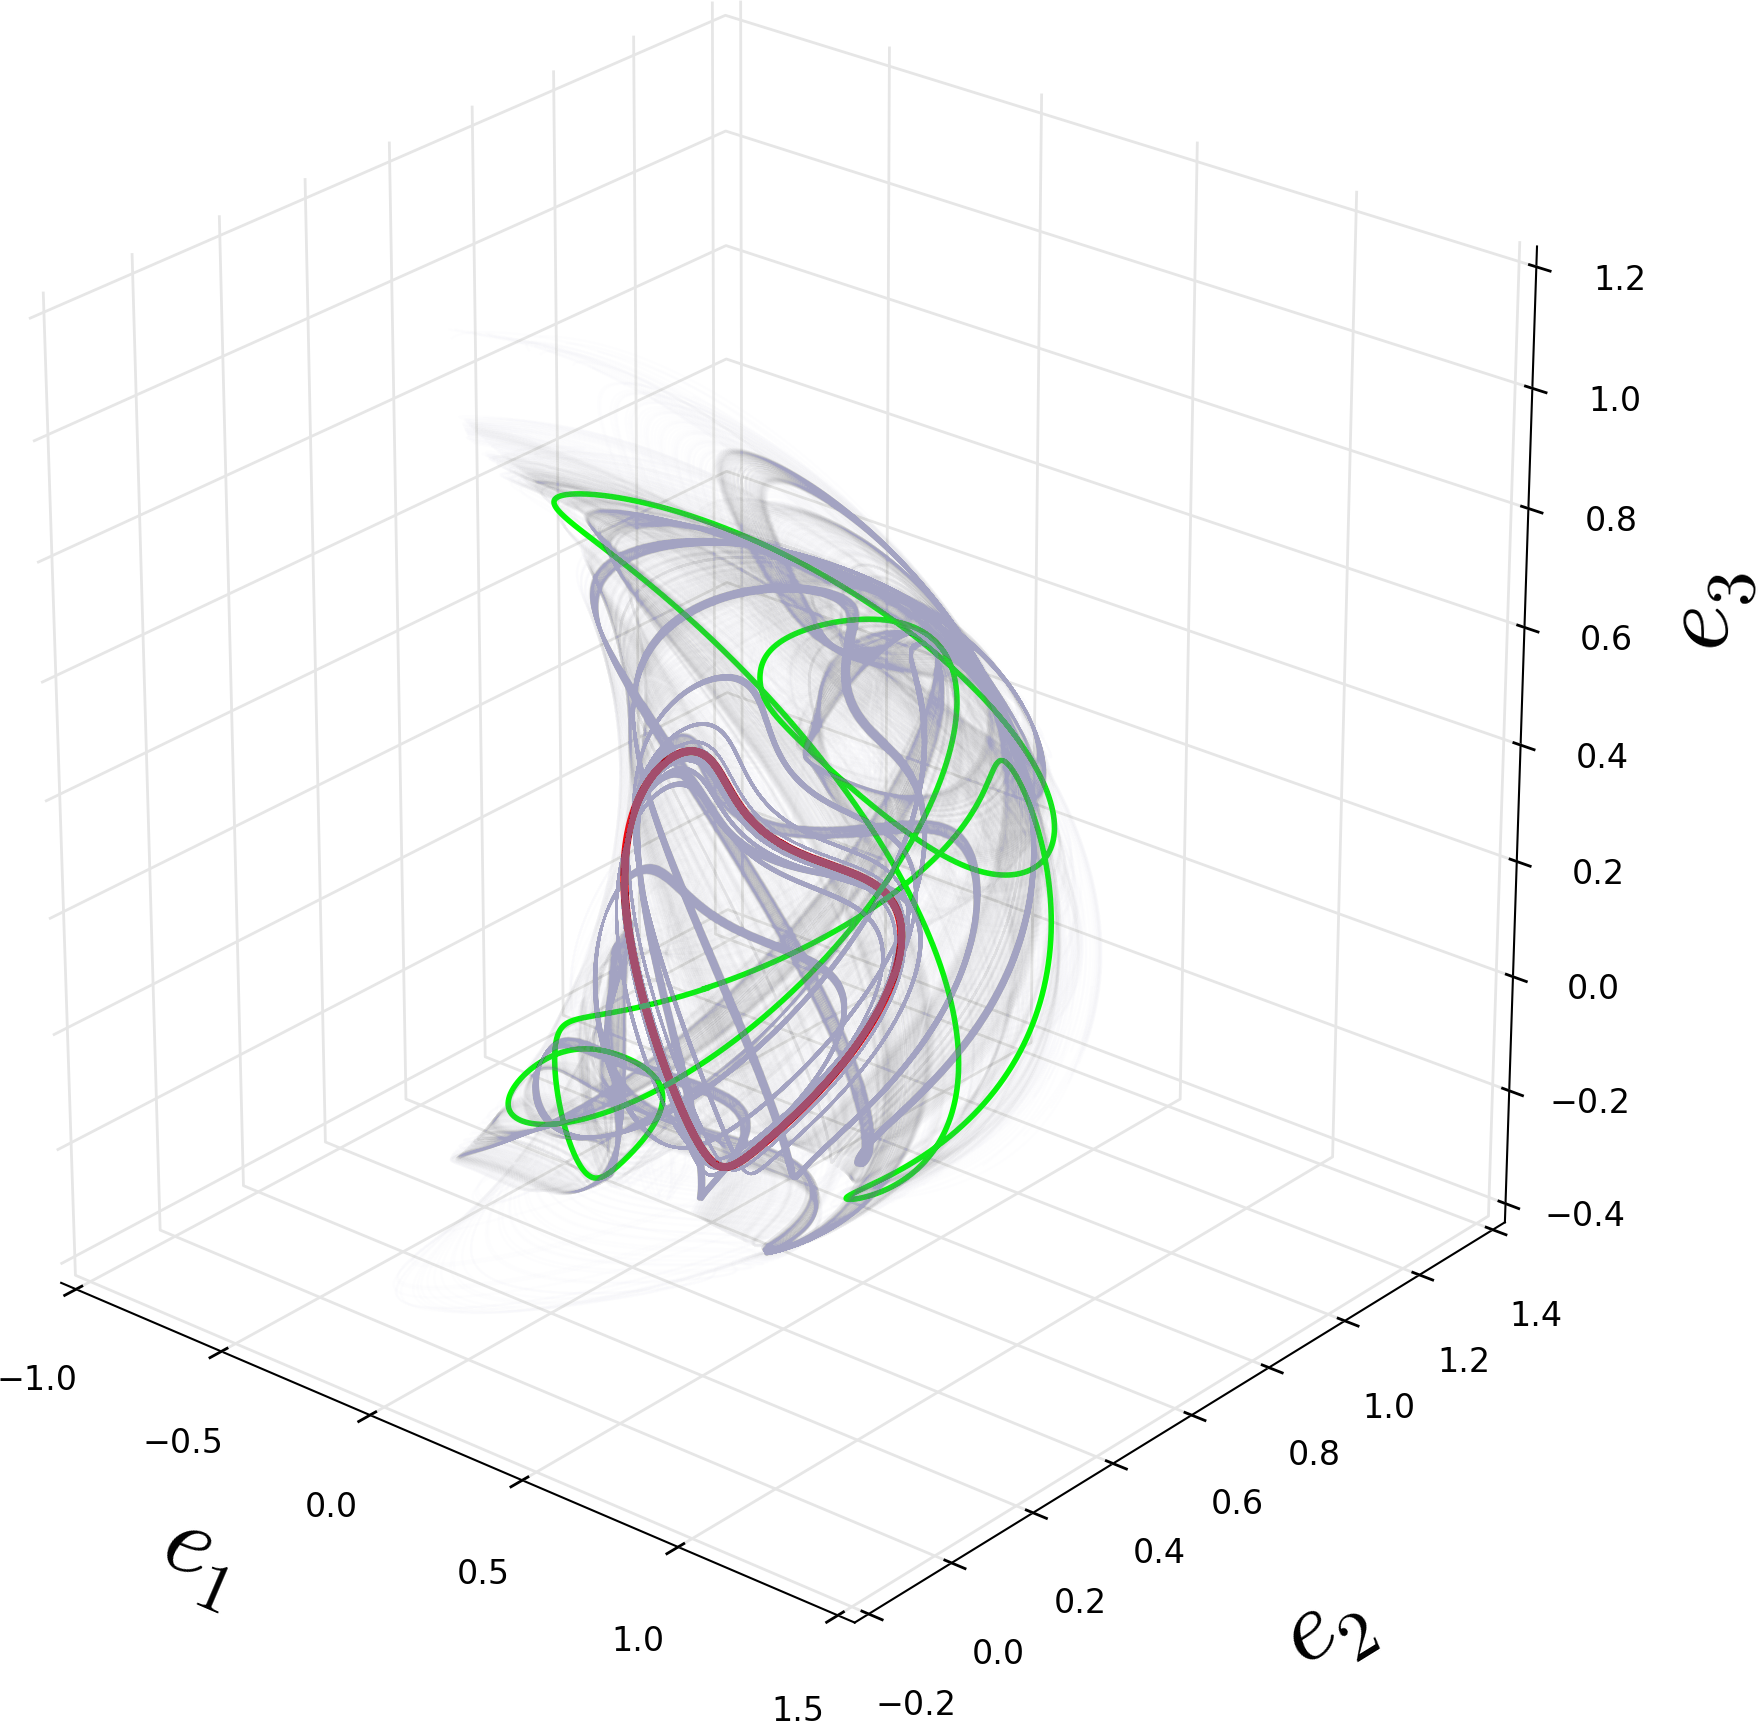
\includegraphics[width=0.40\textwidth]{ksPPO1man3D1}
    (b) 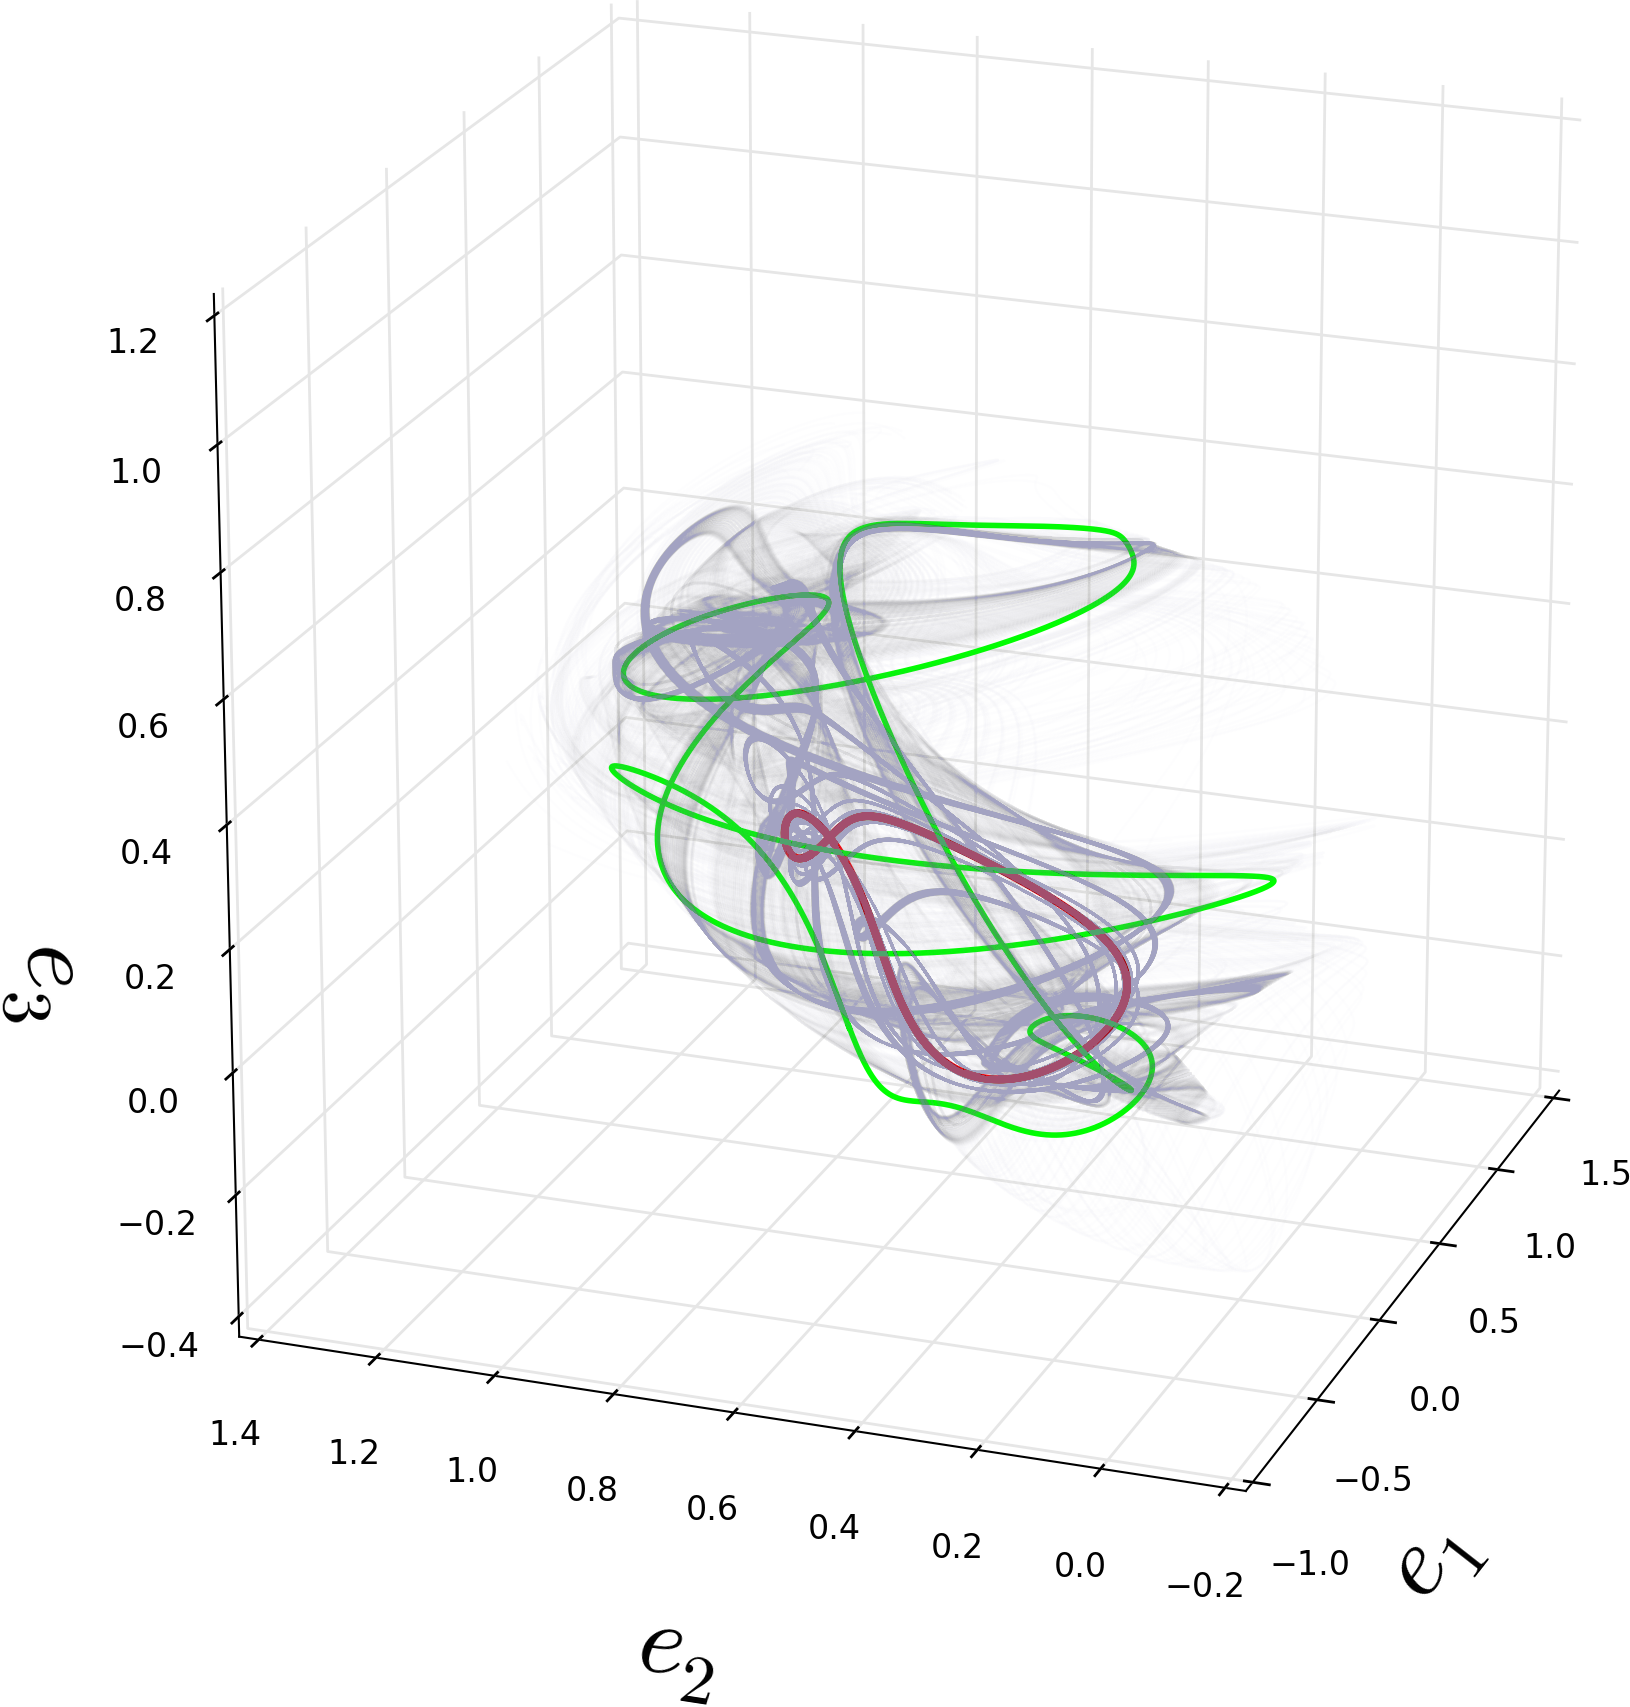
\includegraphics[width=0.40\textwidth]{ksPPO1man3D2}
\end{center}
    \caption[]{
       Unstable manifold of $PPO_{10.3}$ (gray), $PPO_{10.3}$ (red),
       $\RPO{2}=\RPO{32.8}$ (green) projected onto basis formed by
       `Gram-Schmidt'ing
       $e_1 = E_{3, s1}, e_2 = E_{3, s2}, e_3 = E_{2, u}$ with
       $E_{2, s}$ at the origin. (a, b) are two different viewing
       angles.
    }
    \label{f-ksPPO1man3D}
\end{figure}

\item[2015-6-1 Xiong]
I misunderstood what Burak told me last time. I thought the illustration
figure contains ppo2 and rpo1. Since these two shadow each other, the
Floquet vectors should align well. So \reffig{f-ksppo1rpo2} showed the
correct orbits $PPO_{10.3}$ and $\RPO{2}=\RPO{32.8}$ with their Floquet vectors.
Here, O(2) symmetry
is reduced, so the state space is \eqref{e-sspRefRed}. However, it
is still a Fourier mode projection figure. Panel~(a) shows the real
and imaginary part of the leading Floquet vectors. Panel (b) shows
the marginal vector which is used to confirm that my transformation
code is correct. My feeling is that the two orbits are far way and
the Floquet vectors look totally unaligned.
\begin{figure}[ht]
\begin{center}
    (a) 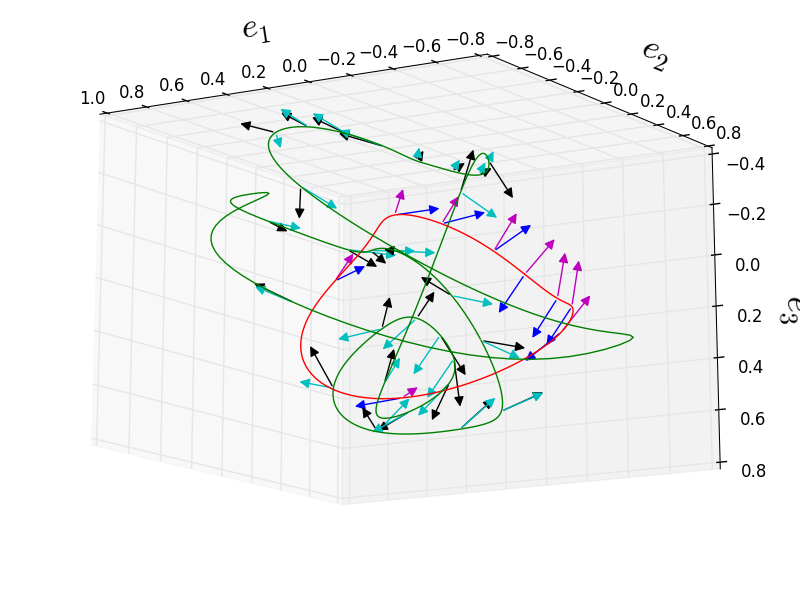
\includegraphics[width=0.45\textwidth]{ppo1rpo2Ve1RealImag}
    (b) 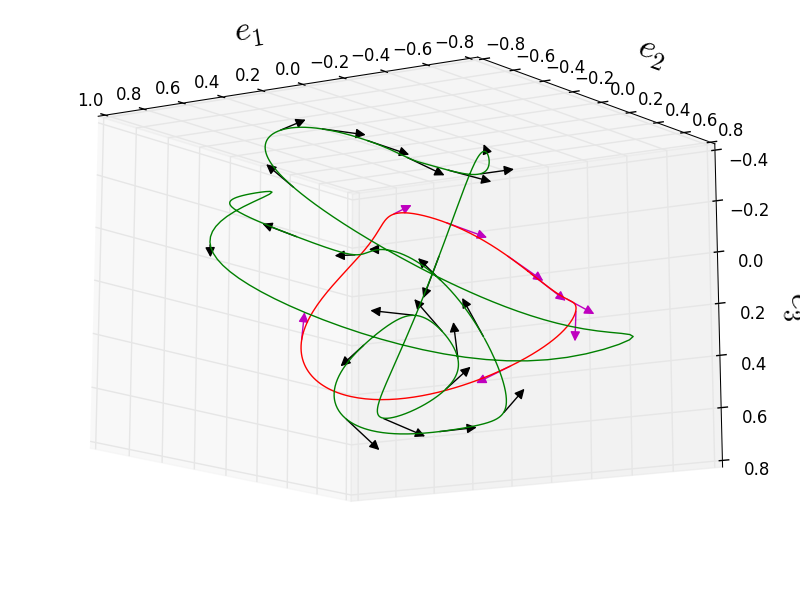
\includegraphics[width=0.45\textwidth]{ppo1rpo2VeMarginal}
\end{center}
    \caption[]{
      (a) $PPO_{10.3}$ (red),$\RPO{2}=\RPO{32.8}$ (green) and the real
      and imaginary part of their leading Floquet vectors long
      the orbit.
      (b) The marginal vector.
    }
    \label{f-ksppo1rpo2}
\end{figure}

\item[2015-06-01 Burak 2 Xiong] It's hard to tell because looking at
first three Fourier mode components show almost nothing. Think of it
this way: There are 30 relevant numbers, and you are making a general
statement by looking at 3 of them. It is true that these orbits far
away, but that is kind of the point here, because
\reffig{f-ksPPO1man3D} shows that the unstable manifold of
$PPO_{10.3}$ extends quite far without its topology
\reffig{f-ppo10p3UnstMan2} breaking down. There is one thing
interesting about \reffig{f-ksppo1rpo2} though, that is, at three
locations I can see, real and imaginary parts of the Floquet vectors
of $\RPO{2}=\RPO{32.8}$ seems to almost overlap. I was expecting this, because
it's probably where they are influenced by a 2 dimensional unstable
manifold, rather than 3D.

Anyways, thanks Xiong, If you don't want to project onto \statesp\
coordinates, I can take it from here to combine \reffig{f-ksPPO1man3D}
and \reffig{f-ksppo1rpo2} if you tell me how to use your code.

\item[2015-6-7 Xiong]
I am trying to replace \reffig{f-ksppo1rpo2} today, but I have
doubts now. To reduce the reflection symmetry, we use
transformation:
$(p_2, p_3) \to  \left(\sqrt{\hat{b}_2^2 + \hat{c}_3^2},
     \frac{\hat{b}_2 \hat{c}_3}{\sqrt{\hat{b}_2^2 + \hat{c}_3^2}}
   \right)\, .
$
The reverse transformation has solution
$\hat{b}_2^2 = \frac{p_2^2 \pm \sqrt{p_2^2 (p_2^2 - 4 p_3^2)}}{2}$.
I just do not understand why one of these two solutions is ruled
out. Also, having 4 pre-images make sense to me, because this
transformation not only reduces reflection symmetry, it also
introduces an additional exchange symmetry, namely, states
with $(\hat{b}_2\,,\hat{c}_3) \to (\hat{c}_3\,,\hat{b}_2)$ will be
reduced to the same state. One alternative transformation could be
$(p_2, p_3) \to  \left(\hat{b}_2^2 - \hat{c}_3^2 \,, \hat{b}_2 \hat{c}_3
   \right)
$, which eliminates the exchange symmetry. It has only 2 pre-images
$\hat{b}_2^2 = \frac{p_2 + \sqrt{p_2^2 + 4 p_3^2}}{2}$.

\item[2015-06-07 Burak] Your argument sounds right, I probably made
a mistake in my previous calculation. Let's switch to
$(p_2, p_3) \to  \left(\hat{b}_2^2 - \hat{c}_3^2 \,, \hat{b}_2 \hat{c}_3
\right)$ then.

\item[2015-06-08 Xiong] We probably could use
$(p_2, p_3) \to
\left(\frac{\hat{b}_2^2 - \hat{c}_3^2}{\sqrt{\hat{b}_2^2 + \hat{c}_3^2}},
     \frac{\hat{b}_2 \hat{c}_3}{\sqrt{\hat{b}_2^2 + \hat{c}_3^2}}
   \right)\, .
$
The inverse transformation is
\[
\hat{b}_2^2 = \frac{p_2^2 + 4p_3^2 \pm \sqrt{p_2^4+4p_2^2p_3^2}}{2} \,,\quad
\hat{c}_3^2 = \frac{p_2^2 + 4p_3^2 \mp \sqrt{p_2^4+4p_2^2p_3^2}}{2}
\]
Whether $\hat{b}_2^2$ or $\hat{c}_3^2$ takes the large solution is
determined by the sign of $p_2$, and whether $\hat{b}_2$ and $\hat{c}_3$
have the same sign or not is determined by the sign of
$p_3$. So there are only 2 pre-images. The modification to the
existing code is minimal.

\item[2015-06-09 Burak] Implemented Xiong's suggestion above, relevant
functions are in \texttt{siminos/ksConnected/} and file names are
\texttt{RefReduce5.m} ,
\texttt{Jacref5.m} ,
\texttt{xtilde2xhat5.m}.
For testing, I reproduced
\reffig{f-ppo10p3UnstMan2} which looks exactly the same
and \reffig{f-ksPPO1man3D} which looks pretty similar in the new
coordinates. \refFig{f-ksPPO1man3D3} is the 3D manifold visualization
at coordinates for reference.
\end{description}

\begin{figure}[ht]
\begin{center}
      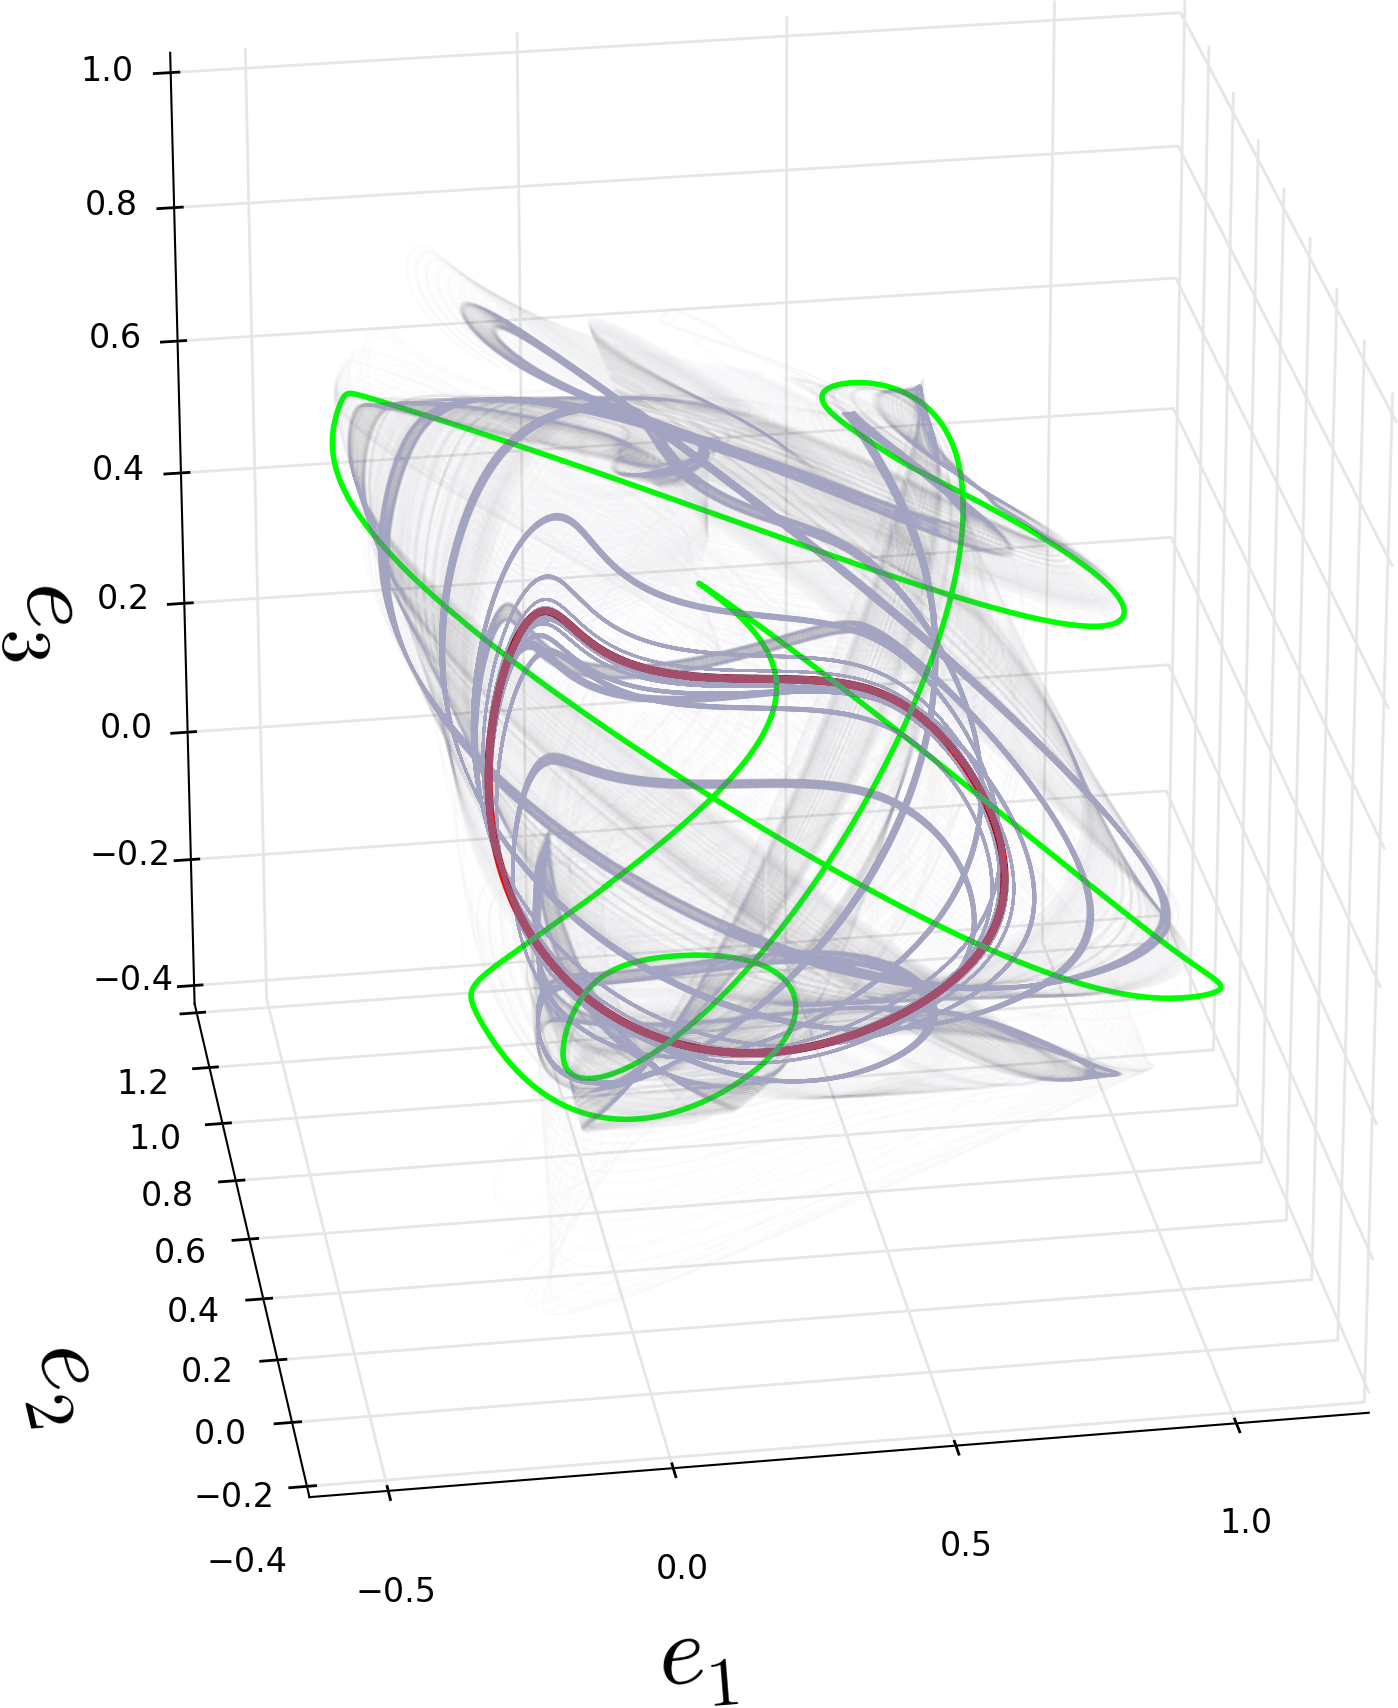
\includegraphics[width=0.45\textwidth]{ksPPO1man3D3}
\end{center}
    \caption[]{
       Unstable manifold of $PPO_{10.3}$ (gray), $PPO_{10.3}$ (red),
       $\RPO{2}=\RPO{32.8}$ (green) projected onto basis formed by
       `Gram-Schmidt'ing
       $e_1 = E_{3, s1}, e_2 = E_{3, s2}, e_3 = E_{2, u}$ with
       $E_{2, s}$ at the origin. (a, b) are two different viewing
       angles.
    }
    \label{f-ksPPO1man3D3}
\end{figure}

\begin{description}

\item[2015-06-15 Burak] I managed to make
\HREF{http://www.matcont.ugent.be/}{matcont} work for numerical
continuation of $PPO_{10.3}$ and my first result is in
\reffig{f-PPO1bifurcation}. Curves in \reffig{f-PPO1bifurcation} (a)
span parameter range $L=(21, 23.32048)$. At the initial point,
$PPO_{10.3}$ is stable and at the final point there is a ``branch
point cycle''. In between, at $L = 21.21912$, there is a
Neimark-Sacker bifurcation, but I'm not sure whether resulting torus
is stable or not. Tomorrow, I'm going to try to follow the branching
point to see if it connects to an RPO, if that is the case, we might
have an explanation for ubiquitous RPO/PPO pairs.

\begin{figure}[ht]
\begin{center}
      (a) 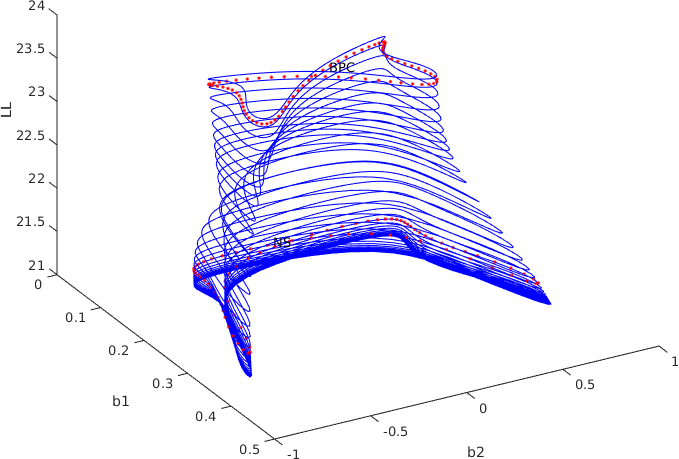
\includegraphics[width=0.55\textwidth]{PPO1bifurcation}
      (b) 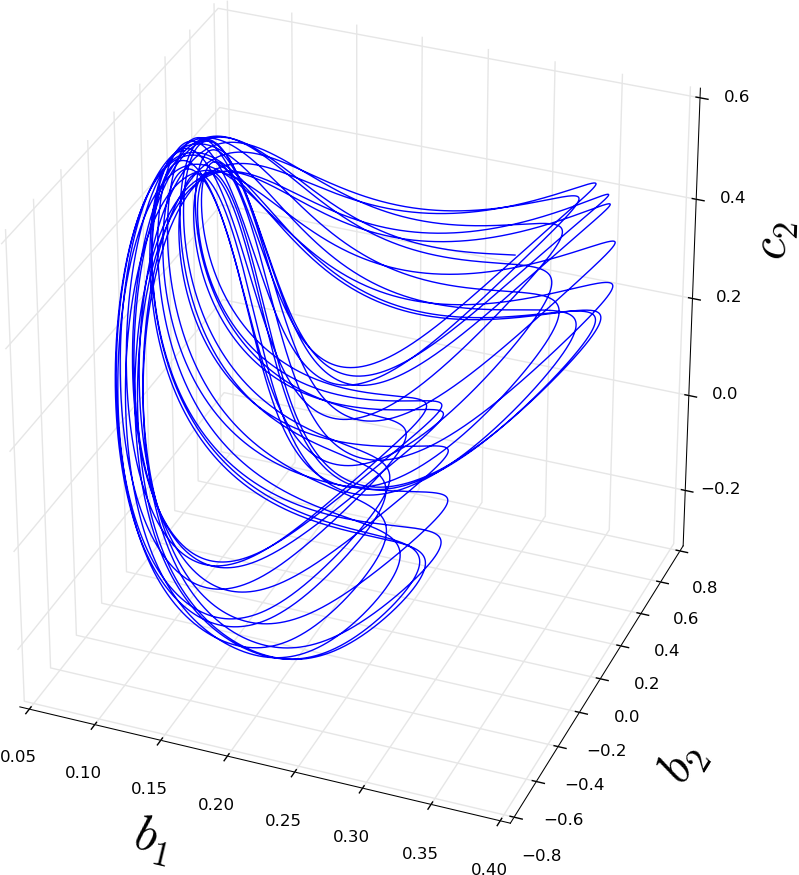
\includegraphics[width=0.35\textwidth]{PPO1torus}
\end{center}
    \caption[]{
       (a) Numerical continuation of $PPO_{10.3}$ starting from $L = 21$
       where it is stable.
       (b) Stable torus bifurcating from $PPO_{10.3}$ at $L=21.21912$.
    }
    \label{f-PPO1bifurcation}
\end{figure}

                                                                    \inCB
\item[2015-06-15 Predrag] In a Hopf (or Poincar\'e-Andronov-Hopf)
bifurcation an \eqv\ point of a continuous-time flow bifurcates into a
(limit) cycle. Local bifurcations of periodic orbits of a continuous-time
flow take place when a Floquet multiplier goes through $|\ExpaEig_j| =1$: (i)
saddle-node bifurcation with multiplier 1, (ii) period doubling
bifurcation with multiplier -1, or (iii) Hopf  (torus)  bifurcation with
a  complex  pair  of Floquet multipliers of unit modulus.

Neimark-Sacker bifurcation (I think) has to do with maps - you would see
it in the \PoincSec\ of the periodic orbit, with a periodic point
bifurcating into a circle. The big deal is avoiding rational resonances - you
yourself have discovered how important avoiding resonances is while
plotting a spiral-out unstable manifold. Of
course, it sounds more important if it has two names attached to it.

                                                                    \inCB
\item[2015-06-15 Burak] When a limit cycle has a complex pair of
Floquet multipliers have unit moduli, \texttt{matcont}
identifies it as an NS bifurcation. I think this is consistent with
your description, since on a \PoincSec\ this would generate a
circle from a fixed point (assuming no rational resonance), which in
the \statesp\ would correspond to a two dimensional torus. Your
definition of Hopf bifurcation for a periodic orbit also describes the
same situation. So I might be wrong in referring to torus bifurcation
of limit cycles as Neimark-Sacker by following
\texttt{matcont}'s classification (supervised by Kuznetsov),
\HREF{http://www.scholarpedia.org/article/Neimark-Sacker_bifurcation\#Torus_Bifurcation}{this remark}
(from article by Kuznetsov and Sacker), and
\HREF{http://www.scholarpedia.org/article/Periodic_orbit\#Bifurcations_Involving_Periodic_Orbits}{this list}
(from article by Moehlis, Josic, and Shea-Brown).
I am not particularly impressed if something has two names attached to
it as opposed to one. In fact, I would prefer to simply call it a
torus bifurcation since it's more informative.

\item[2015-06-16 Xiong] I updated \reffig{f-ksppo1rpo2} with Burak's
coordinates.

\item[2015-06-16 Burak] To see if the torus born out of the bifurcation
of $PPO_{10.3}$ is stable, I integrated a random initial condition at
$L=21.21912$, and the outcome is in \reffig{f-PPO1bifurcation} (b).

\item[2015-06-16 Burak] From the numerical experiments I see that the
torus of \reffig{f-KSTorusL21p3} gets bigger as I increase L, and looses
stability in the transition to chaos.
\refFig{f-KSTorusL21p3} shows the large stable
torus of \KS\ at $L=21.30$, it is unstable at $L=21.31$.

\begin{figure}[ht]
\begin{center}
      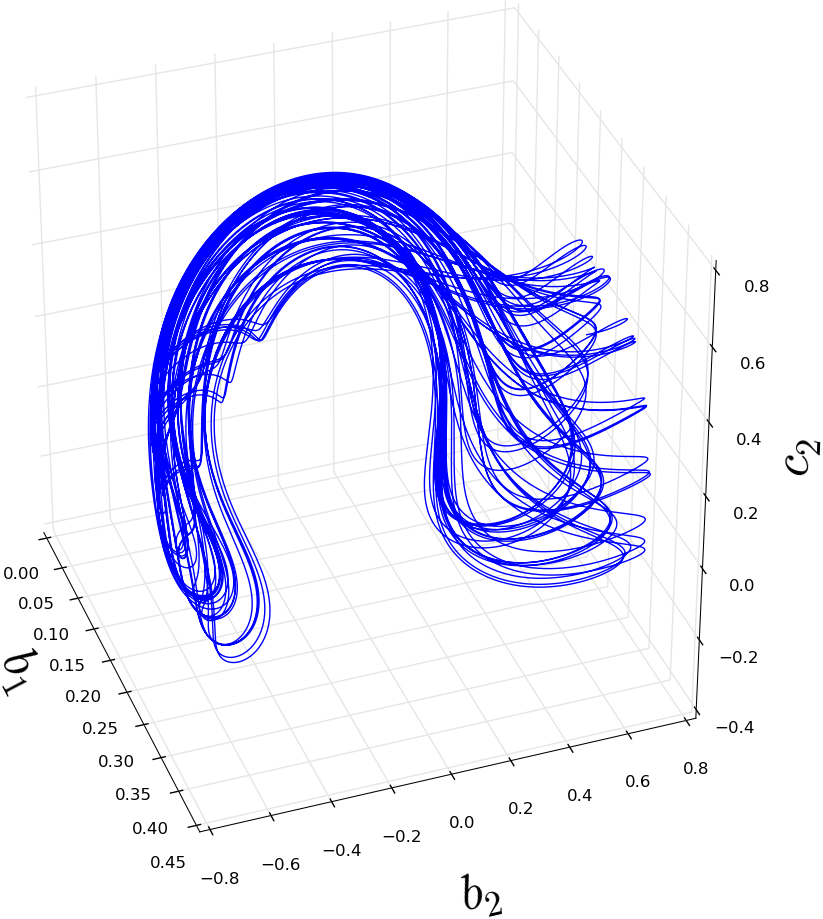
\includegraphics[width=0.45\textwidth]{KSTorusL21p3}
\end{center}
    \caption[]{
       Large stable torus of \KSe\ at $L=21.3$.
    }
    \label{f-KSTorusL21p3}
\end{figure}

\item[2015-07-17 Burak] Following the failure of the cycle expansion attempts,
I diverged a little bit in the \KS\ project. I have some new stuff and I
am going to continue blog them here, since the ultimate goal is to recycle
this.

So I decided to study bifurcations of short periodic orbits and found that the
shortest PPO we know was stable at $L=21$, and bifurcates into a torus at
$L=21.21912$. This torus lives short, and destabilizes at some where close to
$L=21.3$. To get into a bit more detail, I started trajectories as small
perturbations to the periodic orbit in the direction of the real part of the
complex Floquet vector, and looked at them on \PoincSec s.
These orbits are in \reffig{f-PsectL}. Starting from \reffig{f-PsectL} (c),
you can see that the outgoing spirals seem to have three branches.

\begin{figure}
\begin{center}
        (a) 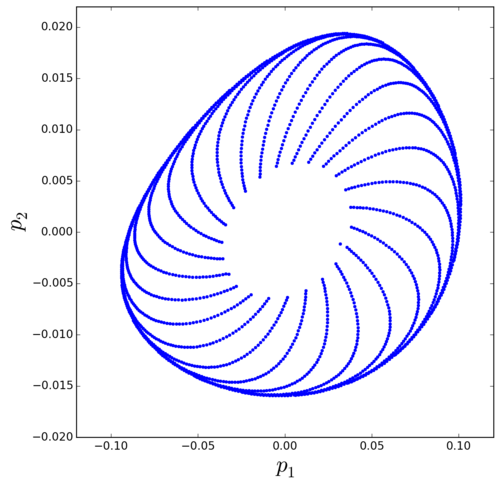
\includegraphics[width=0.30\textwidth]{PsectL21p23}
        (b) 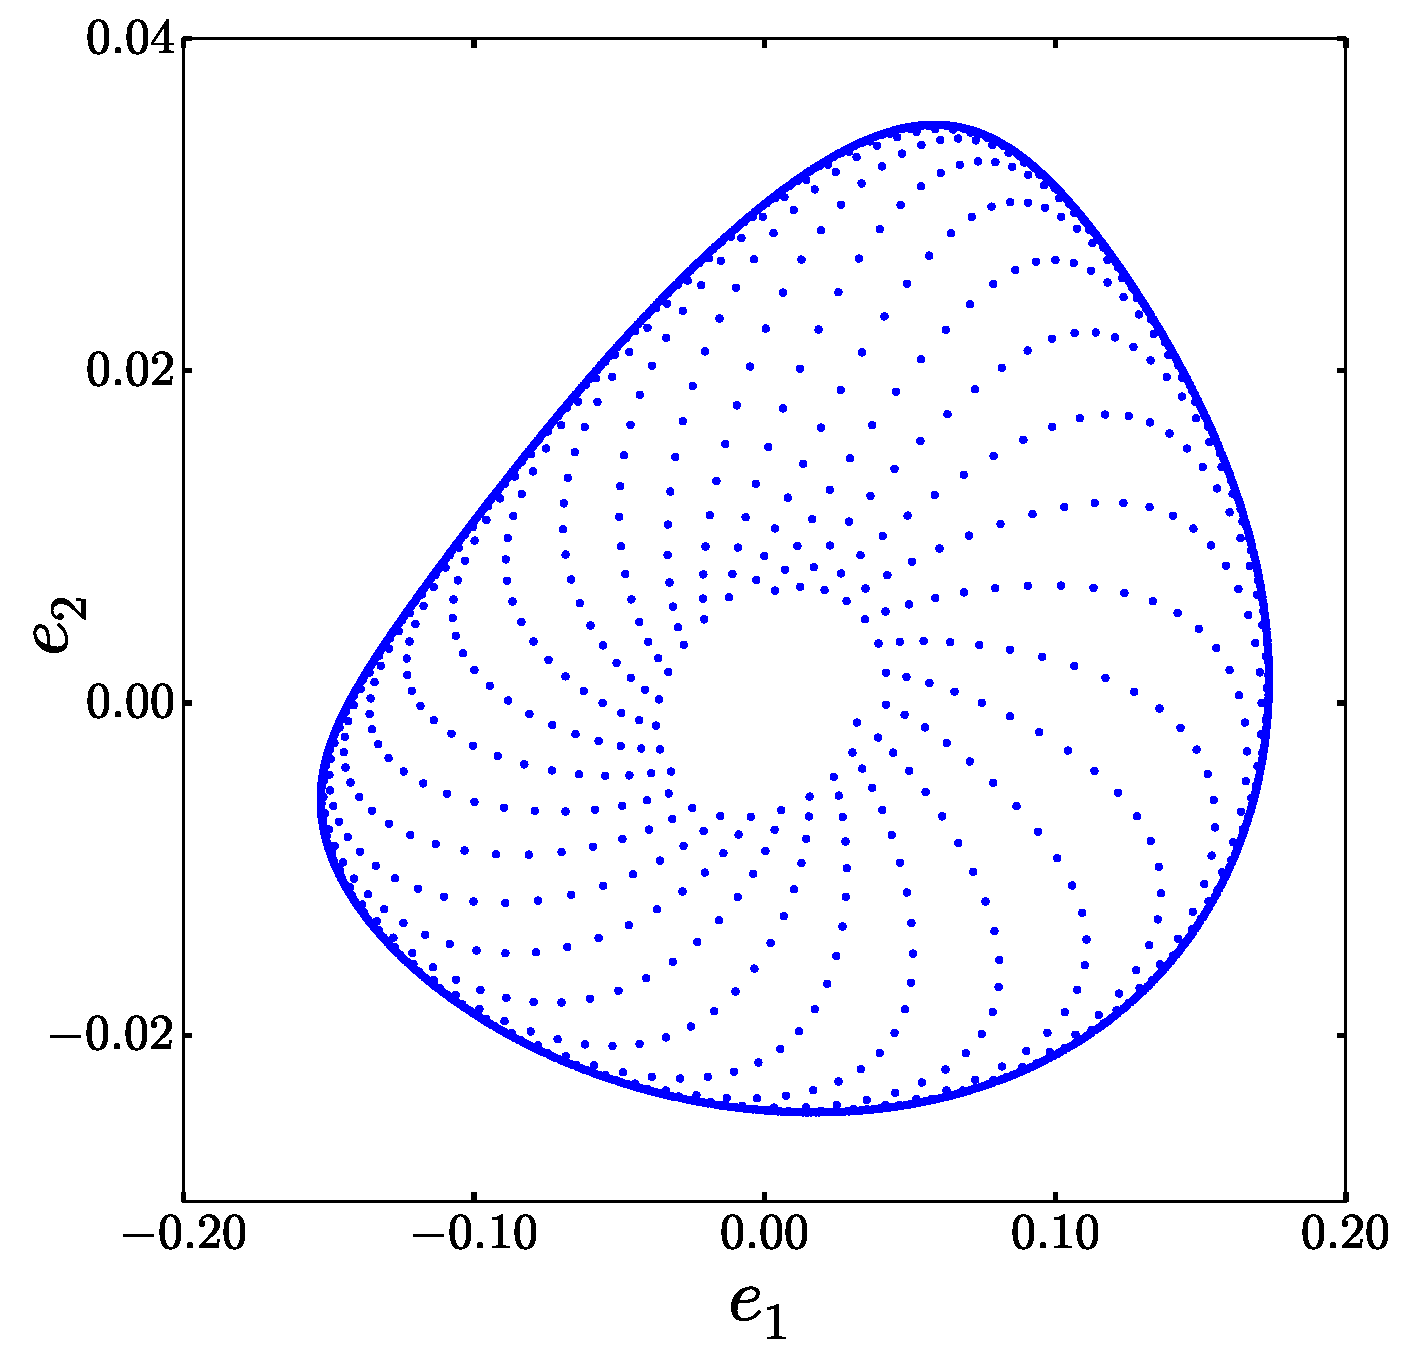
\includegraphics[width=0.30\textwidth]{PsectL21p25}
        (c) 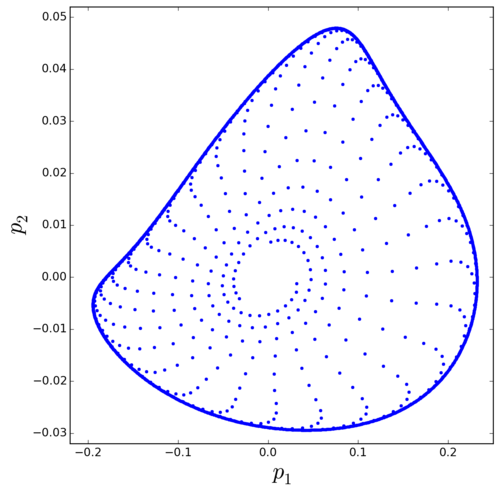
\includegraphics[width=0.30\textwidth]{PsectL21p27} \\
        (d) 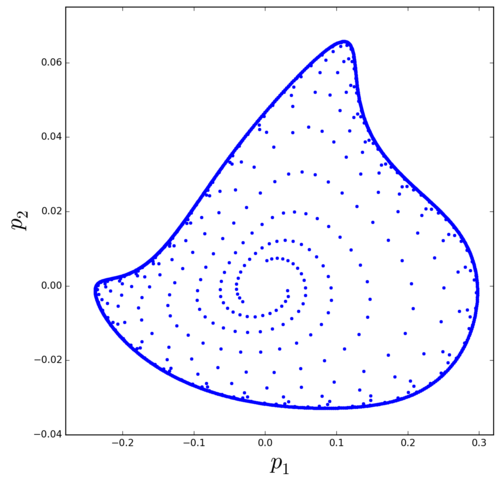
\includegraphics[width=0.30\textwidth]{PsectL21p29}
        (e) 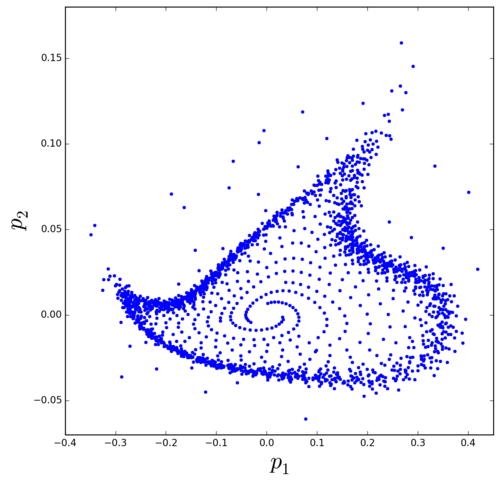
\includegraphics[width=0.30\textwidth]{PsectL21p30}
        (f) 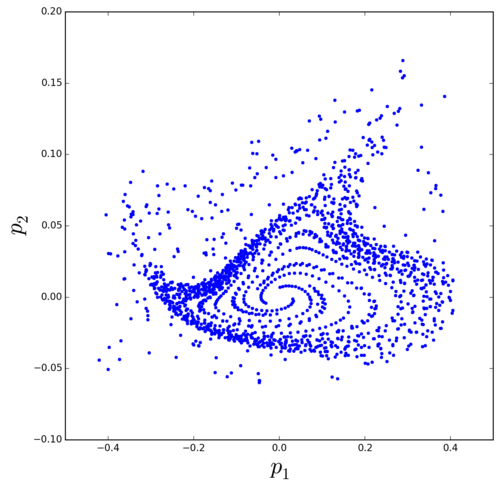
\includegraphics[width=0.30\textwidth]{PsectL21p31}
\end{center}
    \caption{
    \PoincSec\ trajectory of an orbit on the unstable
    manifold of the short PPO after its bifurcation.
    (a) $L = 21.23$ ,
    (b) $L = 21.25$ ,
    (c) $L = 21.27$ ,
    (d) $L = 21.29$ ,
    (e) $L = 21.30$ ,
    (f) $L = 21.31$ ,
    }
    \label{f-PsectL}
\end{figure}

I also plotted the circle maps for these tori, and \reffig{f-CircleMaps} shows
$L=21.29$, which is just before the destabilization of the torus. As you can
see from the map of the third iterate \reffig{f-CircleMaps} (b) that the map
seems to intersect the $\theta_n = \theta_{n+3}$ line. If I take the \statesp\
point corresponding to this value and integrate for three iterates, it comes
really close to itself, and gets closer ($10^{-3}$) after I put it in a Newton
search. However, I haven't managed to converge to this orbit yet. So I'm not
sure this is an exact resonance or near resonance but I'm $99\%$ sure that the
breakdown of the Torus is related to $1\!:\!3$ resonance. Another evidence to this
is the periodic orbits we know at $L=22$, where the shortest orbit has period
$T \approx 10$ and the next shortest orbit within the attractor has period
$T \approx 30$. So I think I can cheat and follow $L=22$ solutions back to find
this orbit exactly but I don't want to do this until I run out of my options.

\begin{figure}
\begin{center}
        (a) 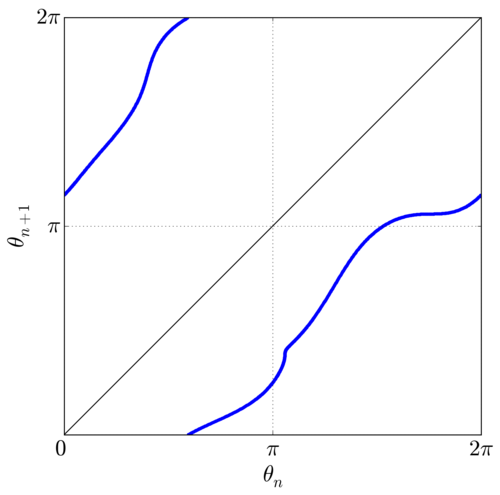
\includegraphics[width=0.45\textwidth]{circleMapL21p29}
        (b) 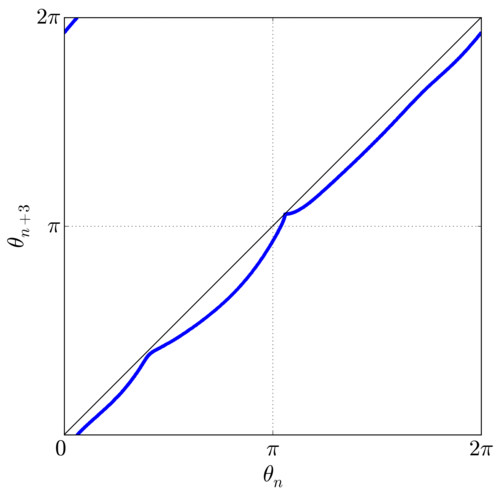
\includegraphics[width=0.45\textwidth]{3rdcircleMapL21p29}
\end{center}
    \caption{
    Poincar\'e return map (a) and its third (b) iterate of the torus at
    $L=21.29$, \reffig{f-PsectL} (d).
    }
    \label{f-CircleMaps}
\end{figure}

% up to here
% former siminos/ksRecycled/tex/blog.tex    master file: BuDiCv15.tex
\item[2015-06-19 Predrag]
\refFig{f-CircleMaps} is ``Poincar\'e return map'', not ``\PoincSec''?
With usual caveats that it is only the angular coordinate of a high-dimensional
return map, and not computed on the unstable manifold, so it might be misleading.

You did not include (c)--(f) figures?\\
\textbf{[2015-07-20 Burak]} I copied caption from the previous figure and
apparently forgot to change it. Fixed it now, sorry for the confusion.

\item[2016-01-10 Predrag]
        	I would like a more radical rewrite, following my draft in pipe blog,
        	explaining Lorenz, \KS, and \NS. In that case nobody can brush of this
        	paper as an ignorant triviality. But you have to get indices
        	worked out first.

\item[2016-01-11 Burak]
        	I don't like the idea of talking about Navier-Stokes symmetry reduction
        	without actually applying it. Even though everything looks fine on
        	equations, there can be all sorts of difficulties when it comes to
        	actually implementing it. We haven't even done the azimuthal part of
        	pipe yet, which I suspect would require time-rescaling. Afterwards,
        	we have to represent data in a spectral way because it does not
        	make sense to multiply finite-element points with each other
        	(we cannot think of different radial points separately, there has to
        	be a single index for all four indices of the velocity field, see
        	pipe blog). For me to be sure about these things, I really have to
        	learn how pipe code works and be able to modify it. Right now, I am
        	working on this but it will take some time. I understand that you
        	want to deemphasize the bifurcation aspect of the paper, but I think
        	it is really important. Guckenheimer \etal\rf{GKOS15} wrote a review
        	on invariant manifolds of equilibria and traveling waves and global
        	bifurcations of $2$ and $3$ dimensional models last year.
        	What we have here are those of \rpo s of a $30$ dimensional
        	discretization of a PDE. I just don't understand why is this not a big
        	deal.


\item[2016-01-10 Predrag]
I was hoping to insert some of the motivational poetry from The Missive,
\refsect{sect:inserts}, into the revised paper, but I failed. When you
resubmit, apologize for the delay - the paper we are resubmitting now is
in content essentially the same as the initial SIADS Manuscript
submission \#M104240 rejected by the editor on Oct 20, 2015, but we have
spent the intervening period in search of this or superior method in the
literature, whose existence was hinted by the editor (with no specific
reference). We have failed to find any such published work, but - in
order not to increase the mean time of refereeing a submission for SIADS
- we propose that this resubmission has a new submission date and a new
SIADS \#M[$\cdots$] .

\item[2016-10-14 Burak to Predrag]
Referee 2 says:

\begin{quote}
3. page 2: "there was no need for heuristic formulations".
Formulations of what?

4. page 2: the first mention of periodic orbit theory
``the formulas of periodic orbit theory that they had formulated in 1983''
is made without an explanation of what this theory is supposed to
describe. May be periodic orbit theory can be deleted from here,
otherwise it needs to be explained here (currently it is done later
in the text).
\end{quote}

I generally agree that the first paragraph is not very clear. I also
do not understand what you meant by
``How they felt about the matter they let on by
referring to these entities as `repulsive cycles'.''
As far as I can see, what \rf{KT84} is missing are zeta functions and
spectral determinants; and ``proof'' that trace formulas hold for
hyperbolic strange sets. For now, I just wrote another paragraph to
further connect study of strange repellers to high dimensional chaos
but I didn't want to touch the first paragraph because it's very
much in your style of writing.

\item[2016-10-16 Burak] Moved the following comment to here as I already
incorporated it:

    \PC{2016-06-25}{
    	I would prefer that \reftab{t-EeigVals} be replaced by the
    	\refref{DingCvit14} notation for Floquet multipliers
    	$ \ExpaEig_i= \exp(\period{}\,\eigRe[i] \pm i\theta_{i})$,
    	and then listing in the $\theta_{i}$ column either the phase, if the
    	Floquet multiplier is complex, or `-1' if the multiplier is real, but
    	inverse hyperbolic ($\arg \ExpaEig_i$ should also be replaced
    	accordingly). That makes the near marginality of
    	$|\ExpaEig_{1,2}|= 1.00636$ easier to understand.
    	That would also, perhaps, make ``symmetry breaking'' bifurcation
    	less mysterious (that's how it works for a parabola).
    }

\item[2016-10-18 Burak] Moving the introduction for recycling

The {exact} weight for a contribution of an unstable periodic orbit to
the escape rate from a strange repeller was given by Kadanoff and
Tang\rf{KT84} in 1983:
\beq
\sum_{x \inFix{n}}
\frac{1}
{\left|\det \left( {\bf 1}-\jMps(x) \right)\right| }
\,,
\label{tr-L0a}
\eeq
where $\jMps(x)$ is the Floquet matrix computed along the orbit of the
periodic point $x$. How they felt about the matter they let on by
referring to these entities as `repulsive cycles'. Since introduction of
zeta functions of Smale (1967)\rf{smale}, Gutzwiller
(1969)\rf{gutzwiller71}, Ruelle (1976)\rf{Ruelle76a, Ruelle76} and their
cycle expansions (1987)\rf{inv} there was no need for heuristic
formulations. Nevertheless, in 1980's something happened that might be
without parallel; this is an area of science where the advent of cheap
computation had actually subtracted from our collective understanding,
with the computer pictures and numerical plots of ``fractal science''
supplanting the deep insights of the 1970's\rf{CBook:appendHist}. But
Kadanoff and Tang, who at the time were  aware only of the work of Bowen
(1975)\rf{bowen}, got it right. Much has happened since -- in particular,
the formulas of periodic orbit theory that they had formulated in 1983
are today at the core of the chalenge very dear to Kadanoff, a dynamical
theory of turbulence\rf{Christiansen97,GHCW07}. For that to work, many
extra moving parts come into play. Among those, taking care of the
symmetries of a nonlinear fluid flow, the focus of this contribution to
Leo P. Kadanoff memorial volume, turns out to be not a trivial problem.

One of the motivations Kadanoff and Tang listed in \rf{KT84}
	for their study of the strange repellers is possibility of having
	such sets as separatrices between different attracting regions of
	larger state spaces. A considerable portion of the recent
	turbulence research
	(see \eg\ \refrefs{TI03, SYE05, SchEckYor07, duguet07, AvMeRoHo13})
	indeed focuses into such subregions of
	state spaces, which separate laminar flow and turbulent
	dynamics. 	
	However, most of these studies relies on physical
	indicators in their analysis, such as kinetic energy or wall
	friction as it is not straightforward to formulate
	symmetry-invariant metrics. Something as simple as measuring
	distances is in fact a challenging problem for a high
	dimensional chaotic system with symmetries.
	First of the two main topics of this paper, the symmetry
	reduction, eliminates this ``degeneracy'' in the \KS\ system
	with \On{2} symmetry. In our following applications, we show
	that the study of unstable manifolds in symmetry-reduced
	state space allows us to find periodic orbits systematically,
	which is a further step towards Kadanoff and Tang's
	proposition of analysing these sets in terms of their cycles.

\item[2016-10-24 Burak] Took out from introduction:

One can express the dynamical averages
(dissipation rates,
diffusion constants, etc.) over the long-time chaotic orbits in terms of
averages computed over the \po s by means of {\Fd s}, and evaluate them
using \cycForm s\rf{DasBuch}. The collection of these methods for
classical and quantum chaos, the \po\  theory, relies heavily on the
understanding of the flow topology and the associated symbolic dynamics.

\item[2016-10-24 Burak] Took out from \refsect{s-SymmRed}:

As a typical example, consider Dhont and
Zhilinski\'i\rf{DhoZhi13,DhoPatZhi15} construction of the classic Weyl
\SOn{2} and \On{2} integrity basis\rf{Weyl39} from
$(x_1,y_1,x_2,y_2,\cdots,x_n,y_n)$ components of $n$ planar vectors. For
two planar vectors there is one syzygy, for three vectors there are 9,
and in the 4-vector case there are already 38 linearly dependent syzygies
of degree 4 in variables $(x_i, y_i)$.

\item[2016-08-18 Predrag] Accidental discovery: Ozorio de Almeida and
Hannay\rf{OzoHan84} in {\em Periodic orbits and a correlation function for
the semiclassical density of states} also gave {exact} weight of an unstable
prime periodic orbit in 1984, in the paragraph after Eq.~(A2.2). Maybe also
reread the paragraph after Eq.~(14) and Eq.~(A1.5). Though their Eq.~(A2.2)
is their usual limit, whereas in ChaosBook these are exact sum rules, no
limit period $ \to \infty$. Who knows, maybe it is older? They do not cite
anyone.

\item[2016-11-22 Predrag]                                       \toCB
Burak and I\rf{BuDiCv15} needed a correct citation for 1942 Hopf bifuraction
paper\rf{hopf42}. Now we have, as well the paper itself\CBlibrary{hopf42}.
It's long paper, so maybe a statement of the theorem in \refref{Hsu76} is useful:
``
The purpose of this paper is to illustrate the simplicity of applying a
theorem of Hopf\rf{hopf42} in establishing the existence of periodic
solutions for the Belousov-Zaikin-Zhabotinskii reaction, and thereby to
publicize Hopf's theorem. This theorem is not as well known and available as
it should be. It is a powerful, direct tool, a general theorem of ordinary
differential equations that directly establishes existence of periodic
solutions to nonlinear systems of orders exceeding 2. It has the
disadvantage, compared to applications of fixed point theorems, that is a
local theorem, local with respect to a parameter. It has the advantage of
possibly leading to a successful analysis of orbital stability.
''

\item[2015-12-02 Predrag]
Is Scholarpedia discusion of the
``\HREF{http://www.scholarpedia.org/article/Equivariant_bifurcation_theory}
{Hopf bifurcation} with \On{2} symmetry'' relevant to our
torus breakdown paper\rf{BudCvi15}?

\item[2015-12-02 Burak]
Scholarpedia equivariant bifurcation theory page discusses only
bifurcation of equilibria, so I don't think it is relevant to our torus
breakdown. However, I think the equilibria of the KS system are the ones
that follow from the equivariant branching lemma.

\item[2015-12-03 Predrag]
Perhaps  Gerard Iooss and Moritz Adelmeyer\rf{IooAde98}
{\em Topics in Bifurcation Theory and Applications}
is relevant to our
torus breakdown paper\rf{BudCvi15}? From the book blurb:
``
... we also study bifurcations (simple here) from group orbits of
solutions in an elementary way (avoiding heavy algebra). The third part
analyzes bifurcations from time periodic solutions of autonomous vector
fields. A normal form theory is developed, covering all cases, and
emphasizing a partial Floquet reduction theory, which is applicable in
infinite dimensions. Studies of period doubling as well as Arnold's
resonance tongues are included in this part.
.''
From
Vanderbauwhede's review\rf{vanderbauwhede_topics_1994}:
``Via an adaptation of Floquet theory it is possible to extend the
foregoing techniques to study bi- furcations near closed orbits,
as is explained in Chapter 3. Next to saddle-point, pitchfork, and Hopf
bifurcations at periodic solutions one also finds period-doubling
bifurcations, while a more detailed analysis of the Hopf bifurcation
leads to the so-called Arnold tongues.''

\item[2015-12-08 Burak]
I'm reading Chossat and Lauterbach once more to be completely safe. It is
a nightmare. Fundamental problem of group theory is the mere fact that
it's incredibly boring. Chapter 7, page 231 says

``We now come to the main results of this section, which are stated in
two theorems."

and then the first theorem says RPOs are tori. Life is too short to be
wasted in formal math, in my wrong opinion.

That being said, I did find one reference from Chossat and Lauterbach
that might contain our invariant polynomials and more. Immediately after
making sure that there is no vector space in Chossat and Lauterbach with
dimensions more than 5, I'll read that one and probably find a generic
way of generating reflection-invariants.

\end{description}
\renewcommand{\ssp}{a}
